\hsection{Mapping Conceptual Entity Types to Logical Models}%
\label{sec:mappingEntitiesToTables}%
%
Translating entity types from the conceptual model to the logical model is fairly simple.
Each entity type in the conceptual model becomes one table in the logical model.
The entity type \emph{Student} becomes the table~\sqlil{student}.
Each simple single-valued attribute becomes one column of that table.
The attribute~\emph{Name} becomes the column~\sqlil{name} with a specific \sql~datatype for text and maybe an added sanity constraint, e.g., names should begin and end with printable (non-whitespace) characters.

Each component of a composite attribute becomes one column of that table.
If \emph{Name} is not a simple attribute but a composite attribute consisting of the two components \emph{Full Name} and \emph{Salutation}, then we will have two columns, one called~\sqlil{full_name} and one called~\sqlil{saluation}.
Both have reasonable datatypes and attached sanity constraints.
In this case, the composite attribute~\emph{Name} in the conceptual model does not have a column in the table for the entity type of the logical model, but instead its components have columns.
Of course, if the components themselves are composite attributes, the process is repeated recursively, i.e., the components are broken down until we arrive at simple attribes, for which we then have columns.

Multivalued attributes come separate tables, where each row references the primary key of entity's table as foreign key.
For example, if the \emph{Student} entity type in the conceptual model has the multivalued attribute \emph{Mobile Phone}, this would mean that each entity of type \emph{Student} can have multiple values of \emph{Mobile Phone} associated with it.
The relational model, all datatypes are atomic, i.e., we cannot have a column that is of type \inQuotes{list of something}.
Each attribute can only have a single value in each record.
Thus, multivalued attributes need to become tables by themselves.
So we would need to create a table~\sqlil{mobile} just for mobile phone numbers.
This table would, at least, need a column for the actual phone number and a column that references the corresponding \emph{Student} record via a foreign key.
It may also need to have a surrogate key, but this we discuss later on.
Derived attributes are not included in the table.

OK, so our goal here would be to either transform the conceptual model of a \db\ to a logical model~(or to directly design the logical model).
But lets first circle back to what a logical model is.
In \cref{def:logicalModel}, we basically stated that the logical model is the collective view that users and applications have on the \db.
In the relational model, this means that it defines all the tables, their attributes and constraints, as well as the queries.

In our small initial example in \cref{sec:simpleExampleFactory}, we only worked with the logical model.
We did not create a conceptual model and neither did we bother with a physical model.
We just directly went for the action, we fired out \sql\ scripts to the \postgresql\ \pgls{server}.
Indeed, if we have chosen an \pgls{rdb} as \db\ type for our project, then the logical model can be specified in \sql\ -- and that is what we did back in that example.

This time, we do have a conceptual model.
We want to follow the \db\ design process properly, based on a software engineering perspective.
Back in \cref{sec:conceptualSchemaDesign}, we designed our conceptual models based on a very loose syntax using the graphical editor \yEd.
This editor is entirely unrelated to any \dbms.
If we wanted, we could have painted diagrams that make no sense at all.
And this freedom is useful when designing conceptual models.
We can quickly change entity types, attributes, and relationships.
We do not need to worry about technical aspects.
We can discuss our model with stakeholders who don't know anything about \sql.

The logical model, however, is bound to a technology.
At this level, using a tool like \yEd\ makes little sense.
Instead, there are also tools that are tied closely to \sql\ or even to specific \pglspl{dbms}.
\mysqlWorkbench~\cite{M2013MWDM}, for example, can connect to the \mysql\ \dbms\ and allows us to craft tables using an \pgls{ERD}\nobreakdashes-like syntax.
\pgmodeler~\cite{AES2006PPDM} allows us to do the same for the \postgresql\ \dbms.
The idea here is that we can use a much clearer and more restricted syntax to draw a visual representation of our \db.
This syntax can then be translated to \sql, which we can send to the \postgresql\ \pgls{server}, e.g., via the \psql\ client.
Using such a \pgls{GUI} has two main advantages:
First, diagrams are intuitive and faster to understand than \sql\ scripts.
Second, the different forms and dialogs that we use to create the \pglspl{ERD} help guiding us to create syntactially correct \sql.

Thus, we first install the \pgmodeler\ as discussed in \cref{sec:installingPgModeler}.
And now, we will try to translate a simple conceptual \pgls{ERD} -- with only a single entity type -- to a logical model.
We use the very first \pgls{ERD} we drew:
the \emph{Student} entity type from \cref{fig:yedErdEntitiesA21erd}.%
%
\begin{figure}%
\centering%
%
\subfloat[][%
A reproduction of the Student \pgls{ERD} from \cref{fig:yedErdEntitiesA21erd}. %
We want to translate this \pgls{ERD} into a logical model for a \db\ that only contains this single table.%
\label{fig:yedErdEntitiesA21erd2}%
]{\includegraphics[width=0.45\linewidth]{\figYedErdEntitiesAXXIerd}}%
%
\floatSep%
%
\subfloat[][%
To start the \pgmodeler, under \ubuntu\ \linux, we open a \pgls{terminal} by hitting \ubuntuTerminal. %
We type in \bashil{pgmodler} and hit~\keys{\enter}. %
Under \microsoftWindows, you would instead proceed as shown in \cref{fig:installingPgModelerWindows22pgmodelerLogo}.%
\label{fig:makeStudentTable01startPgmodeler}%
]{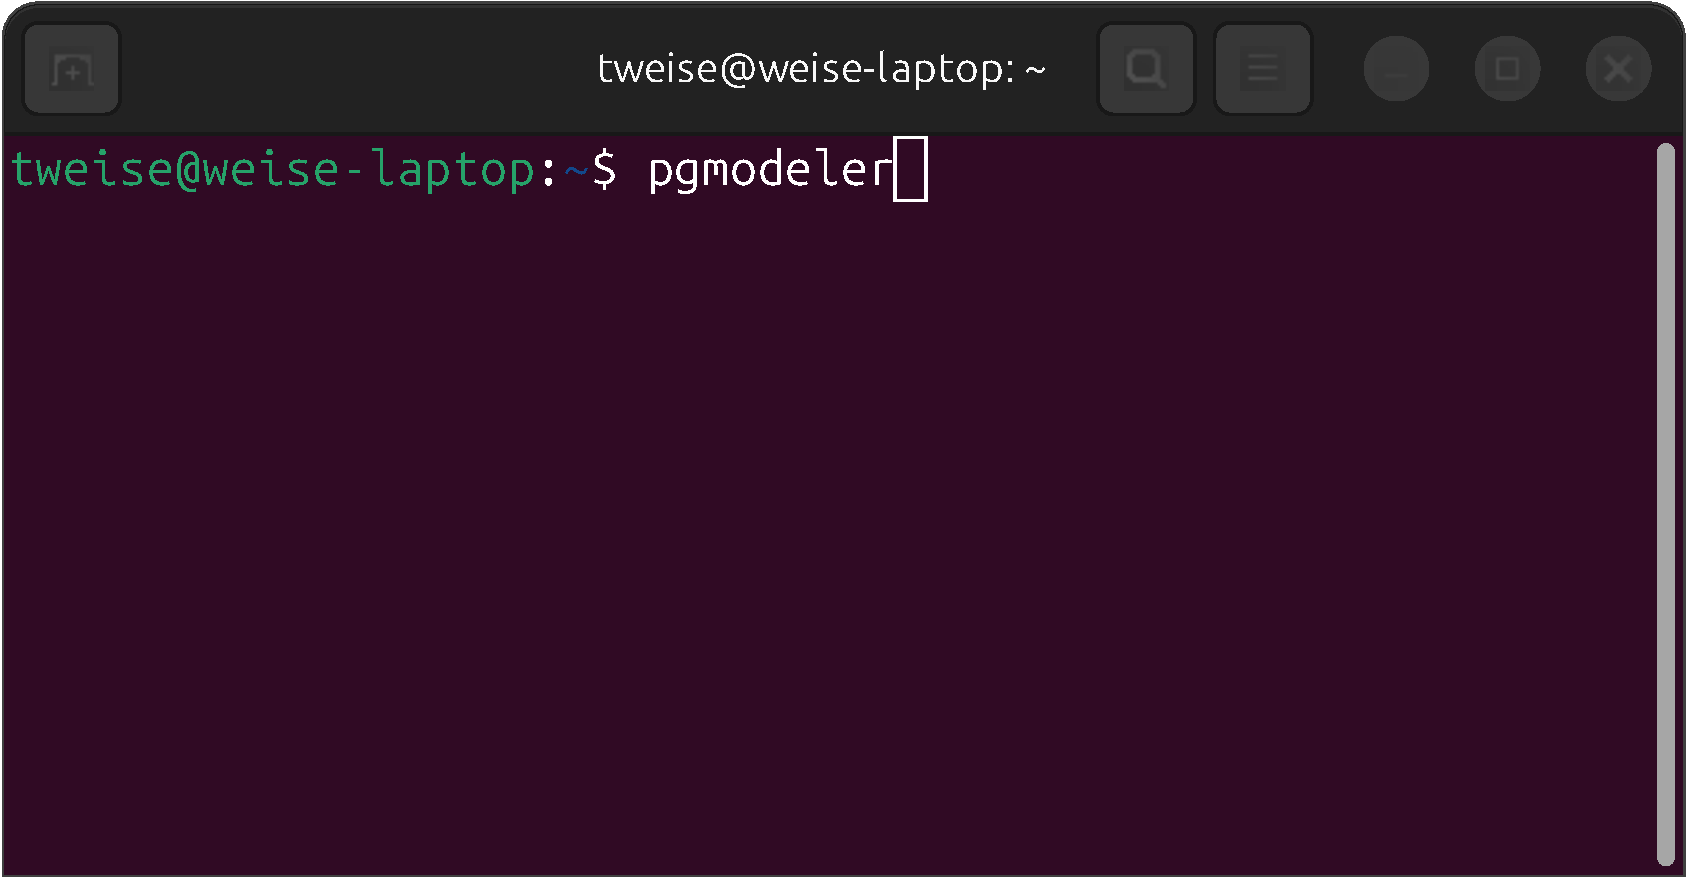
\includegraphics[width=0.53\linewidth]{\currentDir/makeStudentTable01startPgmodeler}}%
%
\floatRowSep%
%
\subfloat[][%
In the \pgmodeler, we click on \menu{New Model}.%
\label{fig:makeStudentTable02newModel}%
]{\tightbox{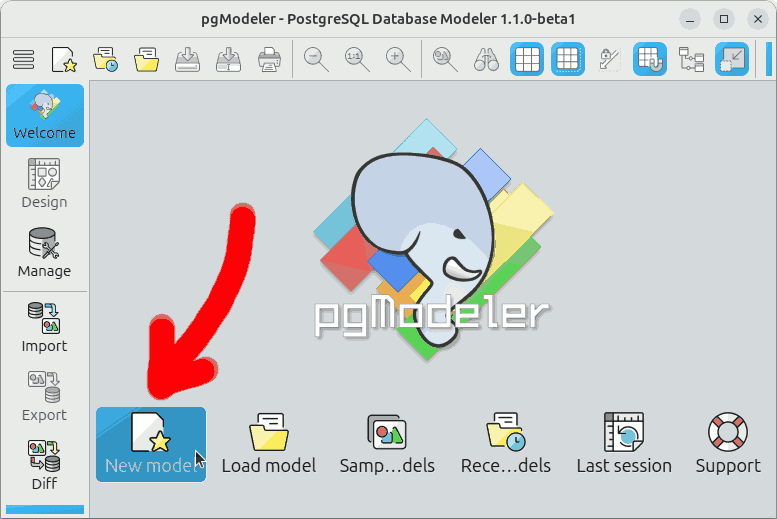
\includegraphics[width=0.48\linewidth]{\currentDir/makeStudentTable02newModel}}}%
%
\floatSep%
%
\subfloat[][%
An empty \pgls{ERD} opens. %
We right-click somewhere in it. %
In the context menu that opens, we click on \menu{Properties}.%
\label{fig:makeStudentTable03rightClickProperties}%
]{\tightbox{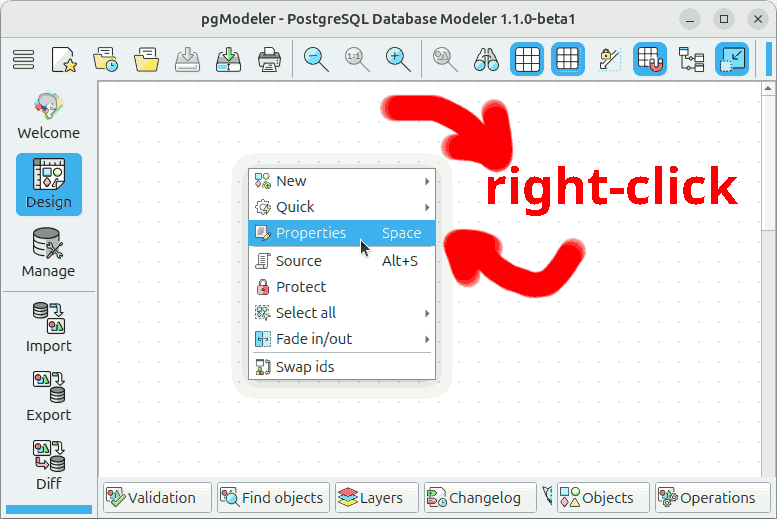
\includegraphics[width=0.48\linewidth]{\currentDir/makeStudentTable03rightClickProperties}}}%
%
\floatRowSep%
%
\subfloat[][%
A dialog called \inQuotes{Database Properties} opens. %
We want to set a proper name for our new \db. %
We choose \sqlil{student_database} and then click on~\menu{Apply}.%
\label{fig:makeStudentTable04propertiesNameApply}%
]{\tightbox{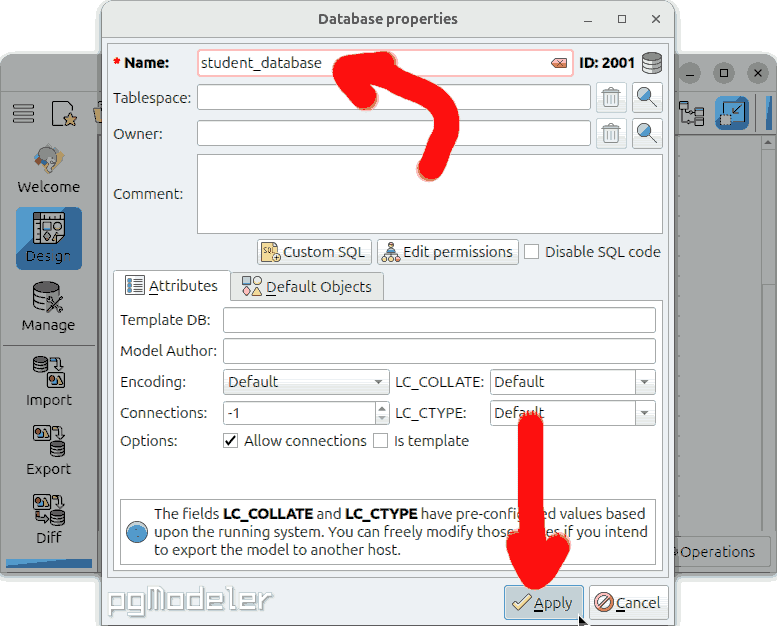
\includegraphics[width=0.48\linewidth]{\currentDir/makeStudentTable04propertiesNameApply}}}%
%
\floatSep%
%
\subfloat[][%
Back in the \pgls{ERD} view, we again right-click into the~(empty) diagram. %
In the popup-menu, we click on~\menu{New>Schema Object>Table}.%
\label{fig:makeStudentTable05newTable}%
]{\tightbox{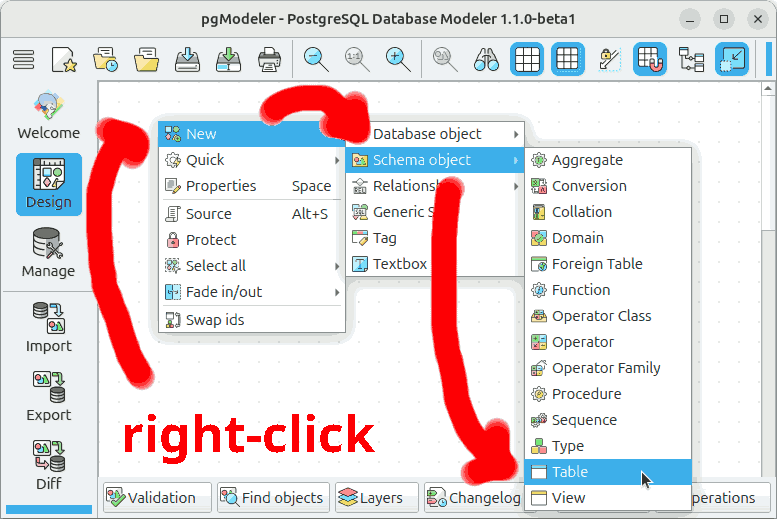
\includegraphics[width=0.48\linewidth]{\currentDir/makeStudentTable05newTable}}}%
%
\label{fig:makeStudentTable:A}%
\caption{Developing logical models using \pgmodeler.}%
\end{figure}%
%
\begin{figure}%
\ContinuedFloat%
\centering%
%
\subfloat[][%
The \inQuotes{Table properties} dialog opens. %
As table name, we enter \sqlil{student}. %
Then we click on the register~\menu{Columns}.%
\label{fig:makeStudentTable06tableNameColumns}%
]{\tightbox{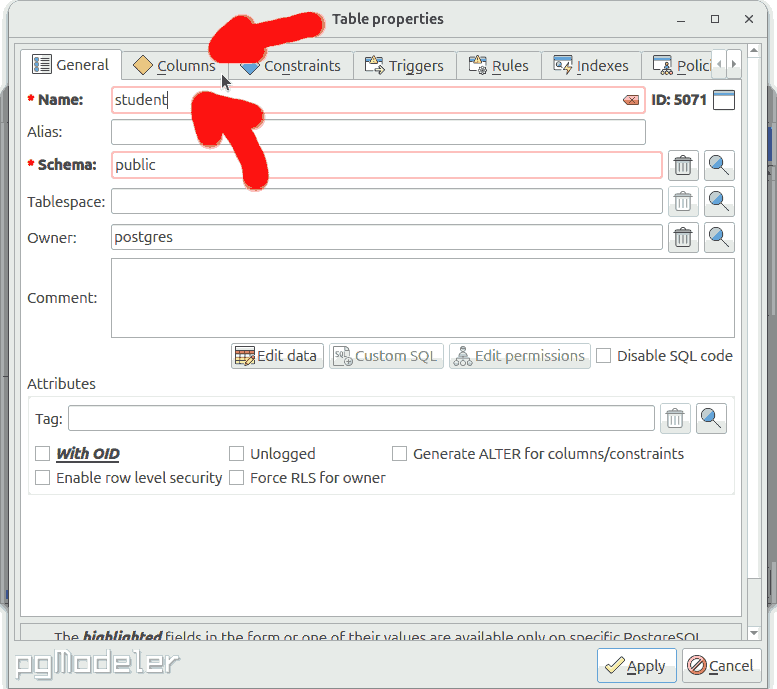
\includegraphics[width=0.48\linewidth]{\currentDir/makeStudentTable06tableNameColumns}}}%
%
\floatSep%
%
\subfloat[][%
In the columns register, we click on the \menu{Add Item} symbol~\pgmodelerAddItem.%
\label{fig:makeStudentTable07newColumn}%
]{\tightbox{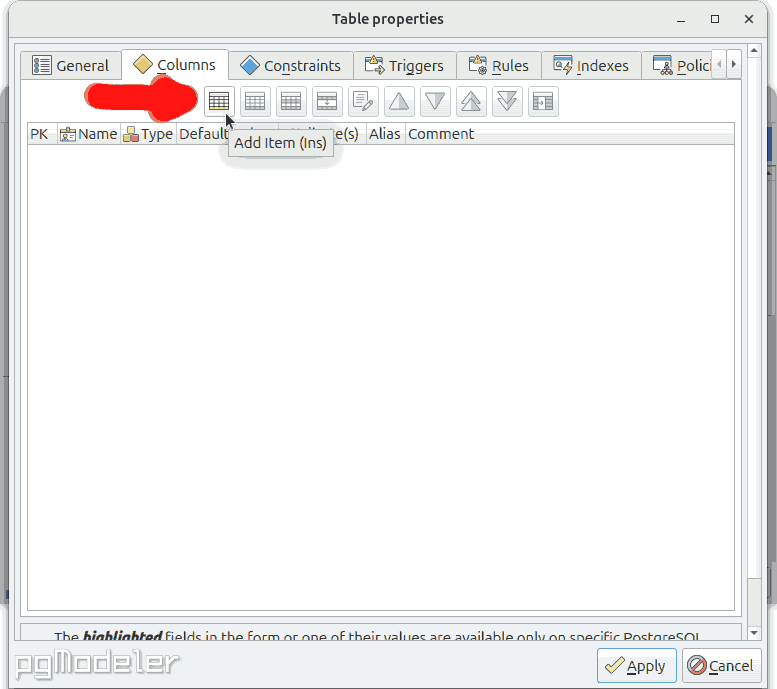
\includegraphics[width=0.48\linewidth]{\currentDir/makeStudentTable07newColumn}}}%
%
\floatRowSep%
%
\subfloat[][%
We want to add a column for the university-issued student~ID. %
As name for this column, we choose~\sqlil{student_id}. %
As type, we choose~\sqlil{character}\sqlIdx{CHARACTER}, i.e., the \sql\ datatype for fixed-length strings~(all student~IDs have the same length).%
\label{fig:makeStudentTable08studentIdNameAndType}%
]{\tightbox{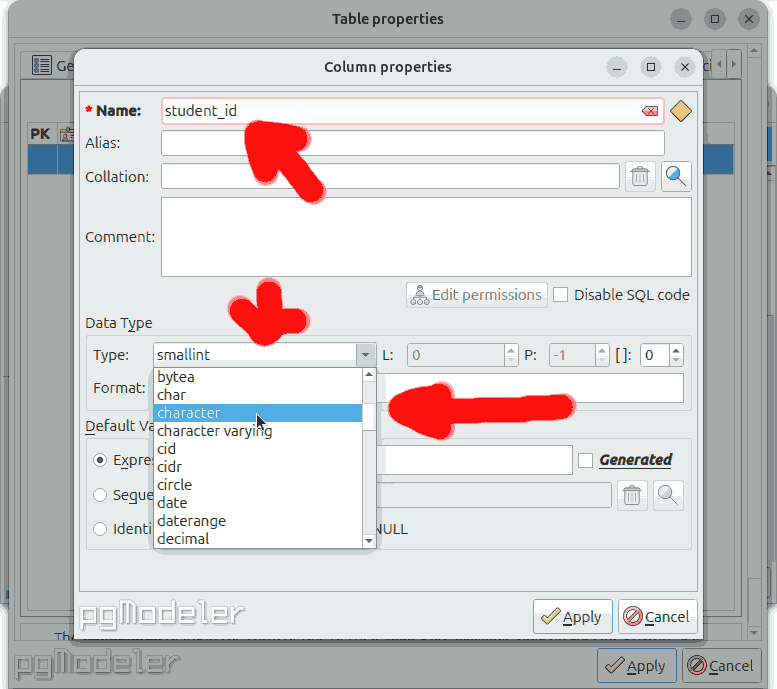
\includegraphics[width=0.48\linewidth]{\currentDir/makeStudentTable08studentIdNameAndType}}}%
%
\floatSep%
%
\subfloat[][%
As~(fixed) length, we enter~11 in the \menu{L:}~field. %
We also mark the column as \sqlilIdx{NOT NULL}, meaning that there cannot be a student record without student~ID. %
We click~\menu{Apply}.%
\label{fig:makeStudentTable09studentIdLenNotNullApply}%
]{\tightbox{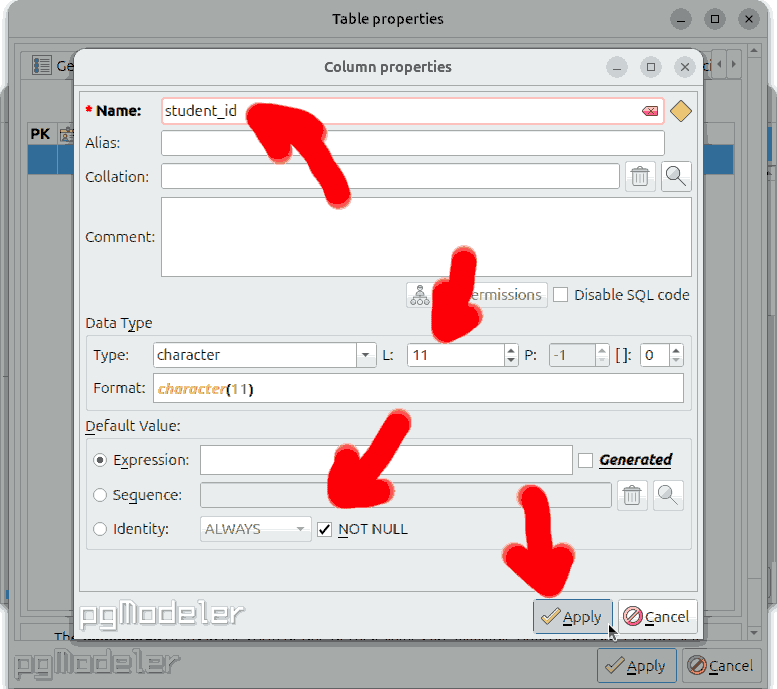
\includegraphics[width=0.48\linewidth]{\currentDir/makeStudentTable09studentIdLenNotNullApply}}}%
%
\label{fig:makeStudentTable:B}%
\caption{Developing logical models using \pgmodeler~(continued).}%
\end{figure}%
%
\begin{figure}%
\ContinuedFloat%
\centering%
%
\subfloat[][%
The new column appears in the dialog. %
We click again on~\menu{Add Item}~\pgmodelerAddItem.%
\label{fig:makeStudentTable10studentIdAddedNewColumn}%
]{\tightbox{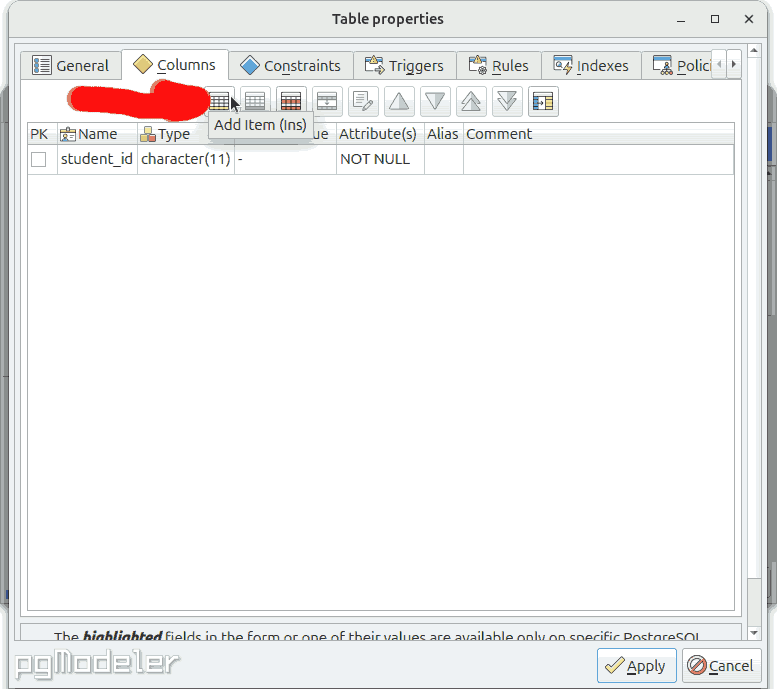
\includegraphics[width=0.48\linewidth]{\currentDir/makeStudentTable10studentIdAddedNewColumn}}}%
%
\floatSep%
%
\subfloat[][%
We add the column \sqlil{national_id} for storing Chinese~ID numbers~(中国公民身份号码). %
Such numbers are strings~(\sqlil{character}\sqlIdx{CHARACTER}) of the fixed length~18. %
We also mark this column as \sqlilIdx{NOT NULL}, meaning that every record must have one. %
We click~\menu{Apply}.%
\label{fig:makeStudentTable11nationalIdNameTypeLenNotNullApply}%
]{\tightbox{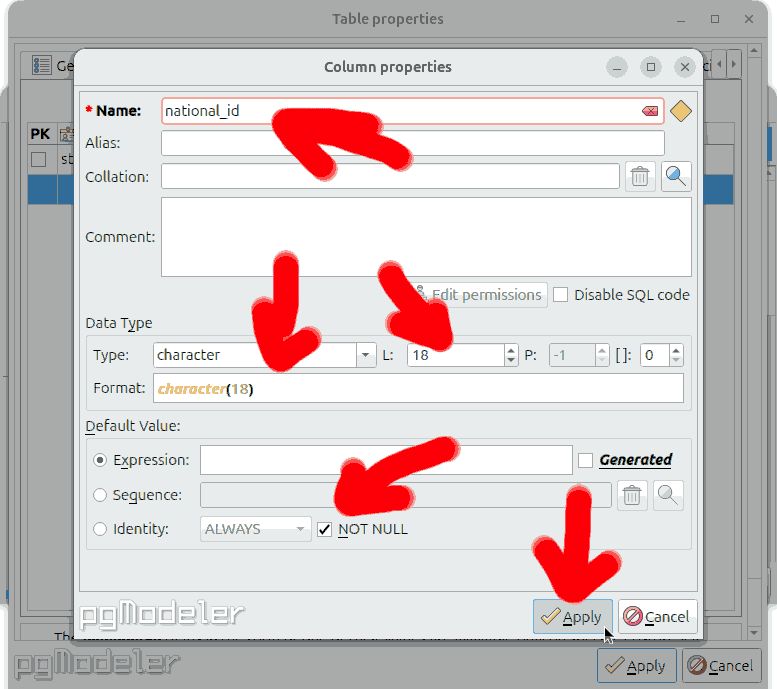
\includegraphics[width=0.48\linewidth]{\currentDir/makeStudentTable11nationalIdNameTypeLenNotNullApply}}}%
%
\floatRowSep%
%
\subfloat[][%
The new column appears and we click~\menu{Add Item}~\pgmodelerAddItem.%
\label{fig:makeStudentTable12nationalIdAddedNewColumn}%
]{\tightbox{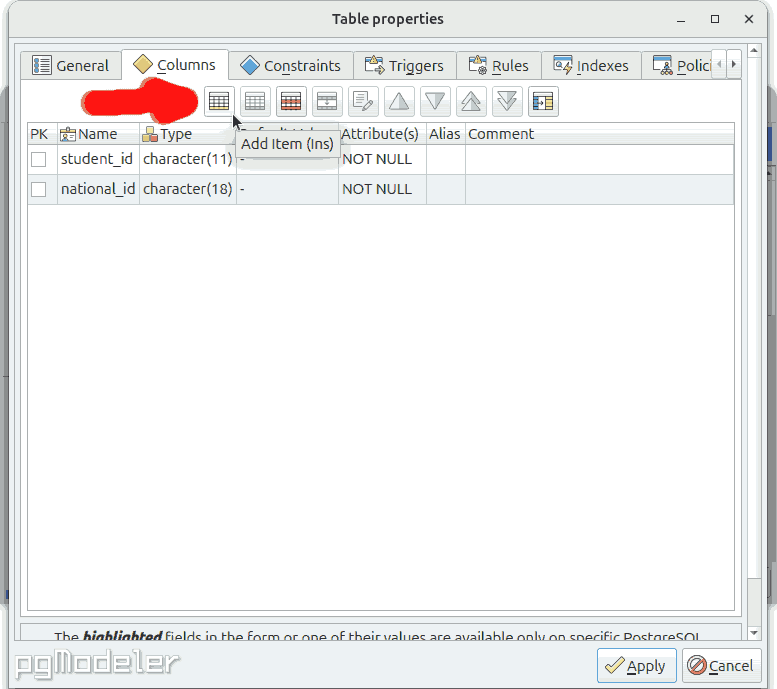
\includegraphics[width=0.48\linewidth]{\currentDir/makeStudentTable12nationalIdAddedNewColumn}}}%
%
\floatSep%
%
\subfloat[][%
We define the column \sqlil{name} for student names. %
Names are of variable length~(type \sqlil{varchar}\sqlIdx{VARCHAR}) and we set the \emph{maximum} length~255. %
Each student must have a name, so we again specify \sqlil{NOT NULL} and click~\menu{Apply}.%
\label{fig:makeStudentTable13nameNameTypeLenNotNullApply}%
]{\tightbox{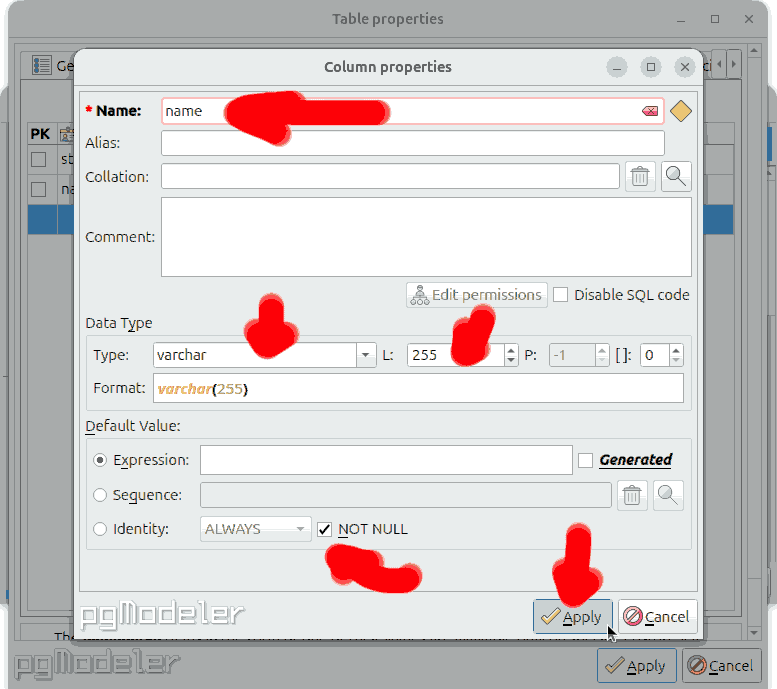
\includegraphics[width=0.48\linewidth]{\currentDir/makeStudentTable13nameNameTypeLenNotNullApply}}}%
%
\label{fig:makeStudentTable:C}%
\caption{Developing logical models using \pgmodeler~(continued).}%
\end{figure}%
%
\begin{figure}%
\ContinuedFloat%
\centering%
%
\subfloat[][%
The new column appears in the dialog. %
We click again on~\menu{Add Item}~\pgmodelerAddItem.%
\label{fig:makeStudentTable14nameAddedNewColumn}%
]{\tightbox{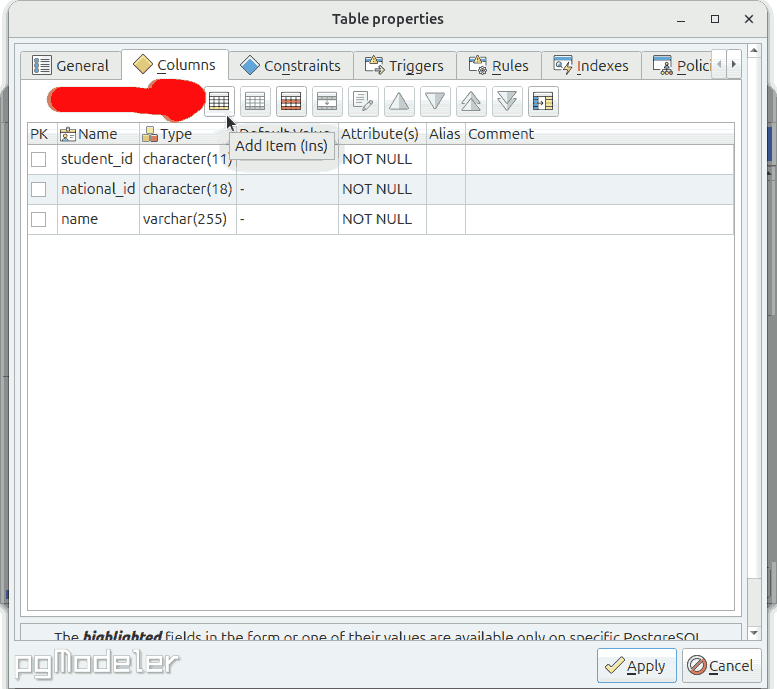
\includegraphics[width=0.48\linewidth]{\currentDir/makeStudentTable14nameAddedNewColumn}}}%
%
\floatSep%
%
\subfloat[][%
Addresses, too, are strings of variable length~(type \sqlil{varchar}\sqlIdx{VARCHAR}). %
We again set the maximum length to~255, require the field to be \sqlilIdx{NOT NULL}, and click~\menu{Apply}.%
\label{fig:makeStudentTable15addressNameTypeLenNotNullApply}%
]{\tightbox{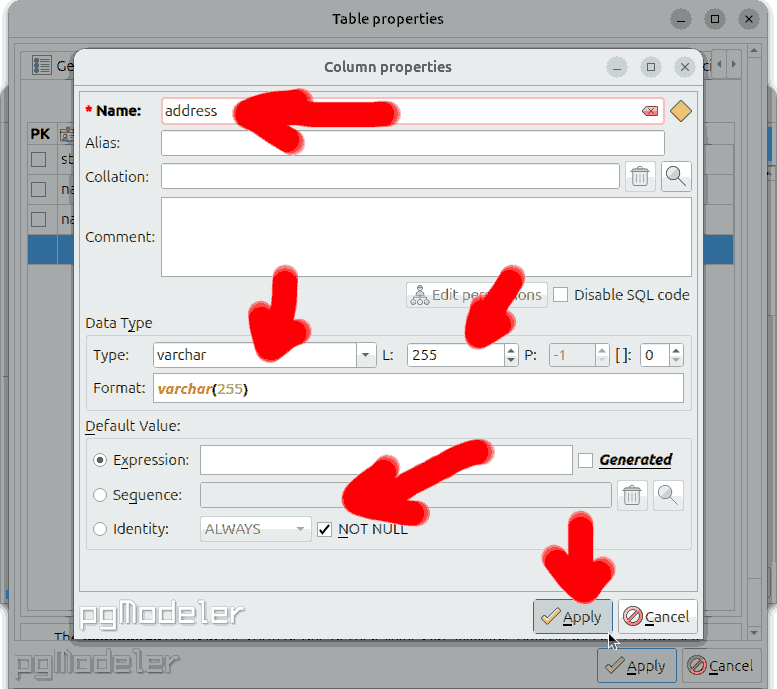
\includegraphics[width=0.48\linewidth]{\currentDir/makeStudentTable15addressNameTypeLenNotNullApply}}}%
%
\floatRowSep%
%
\subfloat[][%
The new column appears and we click~\menu{Add Item}~\pgmodelerAddItem.%
\label{fig:makeStudentTable16addressAddedNewColumn}%
]{\tightbox{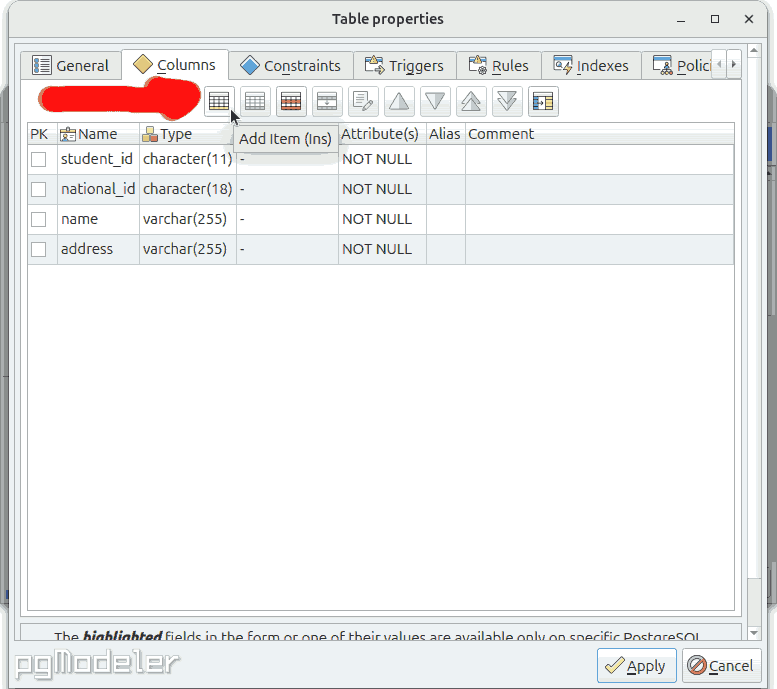
\includegraphics[width=0.48\linewidth]{\currentDir/makeStudentTable16addressAddedNewColumn}}}%
%
\floatSep%
%
\subfloat[][%
We now add a column for \sqlil{mobile} phone numbers. %
In China, these are strings~(\sqlil{character}\sqlIdx{CHARACTER}) of the fixed length~11. %
We require that they must be specified~(\sqlilIdx{NOT NULL}) and click~\menu{Apply}.%
\label{fig:makeStudentTable17mobileNameTypeLenNotNullApply}%
]{\tightbox{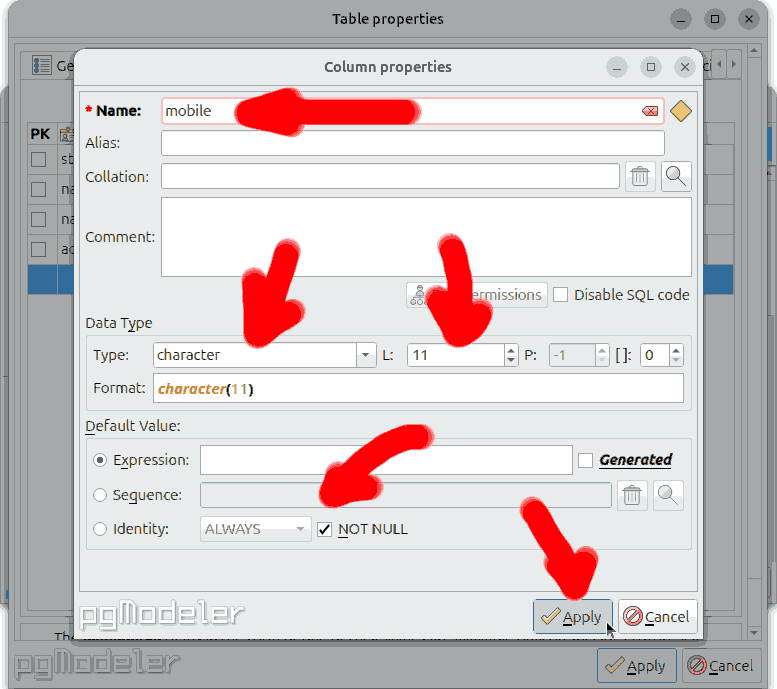
\includegraphics[width=0.48\linewidth]{\currentDir/makeStudentTable17mobileNameTypeLenNotNullApply}}}%
%
\label{fig:makeStudentTable:D}%
\caption{Developing logical models using \pgmodeler~(continued).}%
\end{figure}%
%
\begin{figure}%
\ContinuedFloat%
\centering%
%
\subfloat[][%
The new column appears in the dialog. %
We click again on~\menu{Add Item}~\pgmodelerAddItem.%
\label{fig:makeStudentTable18mobileAddedNewColumn}%
]{\tightbox{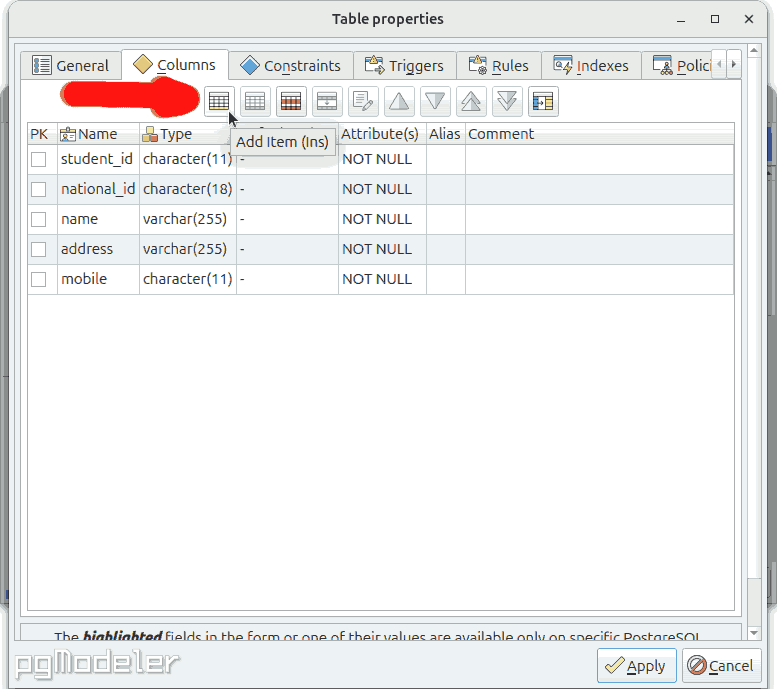
\includegraphics[width=0.48\linewidth]{\currentDir/makeStudentTable18mobileAddedNewColumn}}}%
%
\floatSep%
%
\subfloat[][%
Finally, we add the \glsreset{dateOfBirth}\pgls{dateOfBirth} in form of a \sqlil{date_of_birth} column. %
The type here is \sqlil{date}\sqlIdx{DATE} and \pglspl{dateOfBirth} are required to be \sqlilIdx{NOT NULL}. %
We click~\menu{Apply}.%
\label{fig:makeStudentTable19dateOfBirthNameTypeNotNullApply}%
]{\tightbox{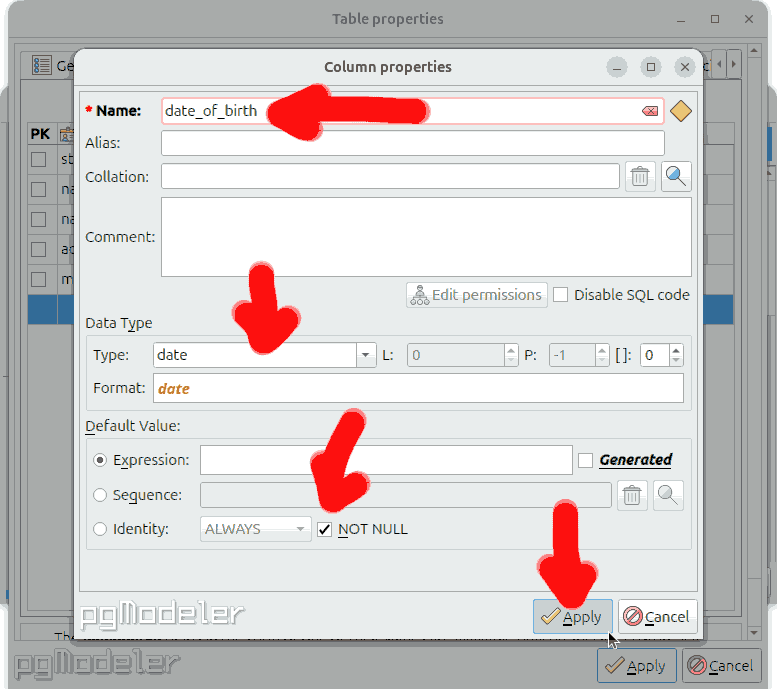
\includegraphics[width=0.48\linewidth]{\currentDir/makeStudentTable19dateOfBirthNameTypeNotNullApply}}}%
%
\floatRowSep%
%
\subfloat[][%
The new column appears. %
We click on the register \menu{Constraints}, because now we want to add validity rules for our data.%
\label{fig:makeStudentTable20dateOfBirthAddedConstraints}%
]{\tightbox{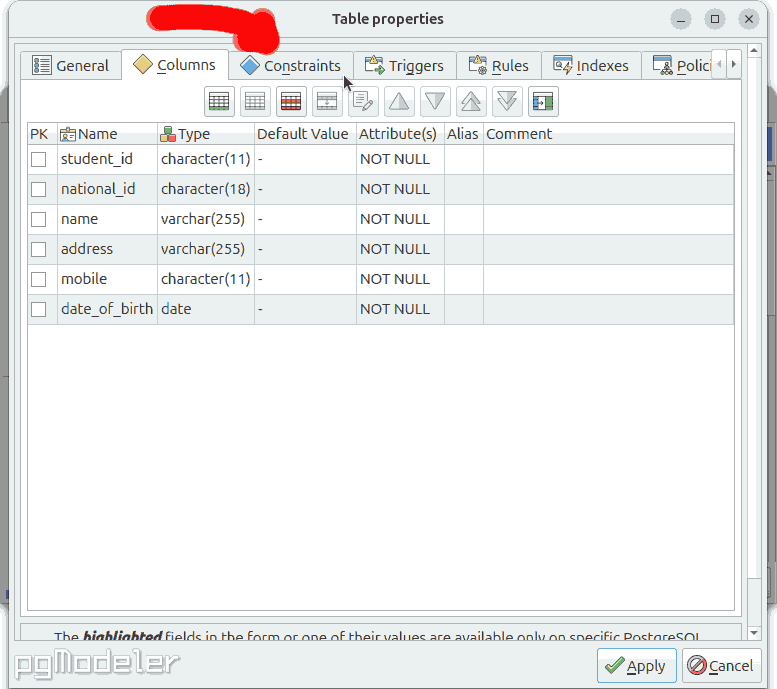
\includegraphics[width=0.48\linewidth]{\currentDir/makeStudentTable20dateOfBirthAddedConstraints}}}%
%
\floatSep%
%
\subfloat[][%
In the \menu{Constraints} register, we click~\menu{Add Item}~\pgmodelerAddItem.%
\label{fig:makeStudentTable21newConstraint}%
]{\tightbox{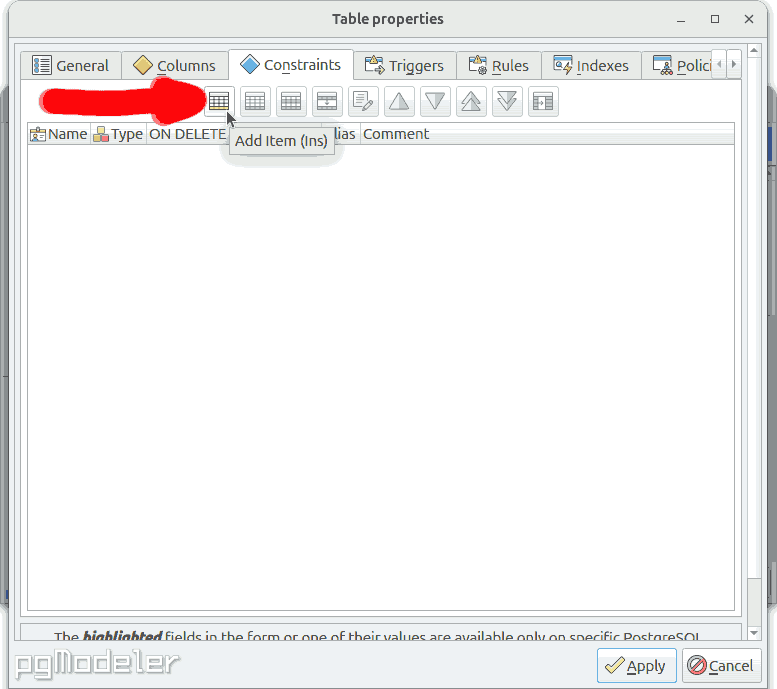
\includegraphics[width=0.48\linewidth]{\currentDir/makeStudentTable21newConstraint}}}%
%
\label{fig:makeStudentTable:E}%
\caption{Developing logical models using \pgmodeler~(continued).}%
\end{figure}%
%
\begin{figure}%
\ContinuedFloat%
\centering%
%
\subfloat[][%
As first constraint, we want to define \sqlil{student_id} as the primary key of our table. %
We call this constraint \sqlil{student_student_id_pk} and select \sqlilIdx{PRIMARY KEY} as type. %
We select the column \sqlil{student_id} in the \menu{Column} drop-down box and click on~\menu{Add Item}~\pgmodelerAddItem.%
\label{fig:makeStudentTable22studentIdPkData}%
]{\tightbox{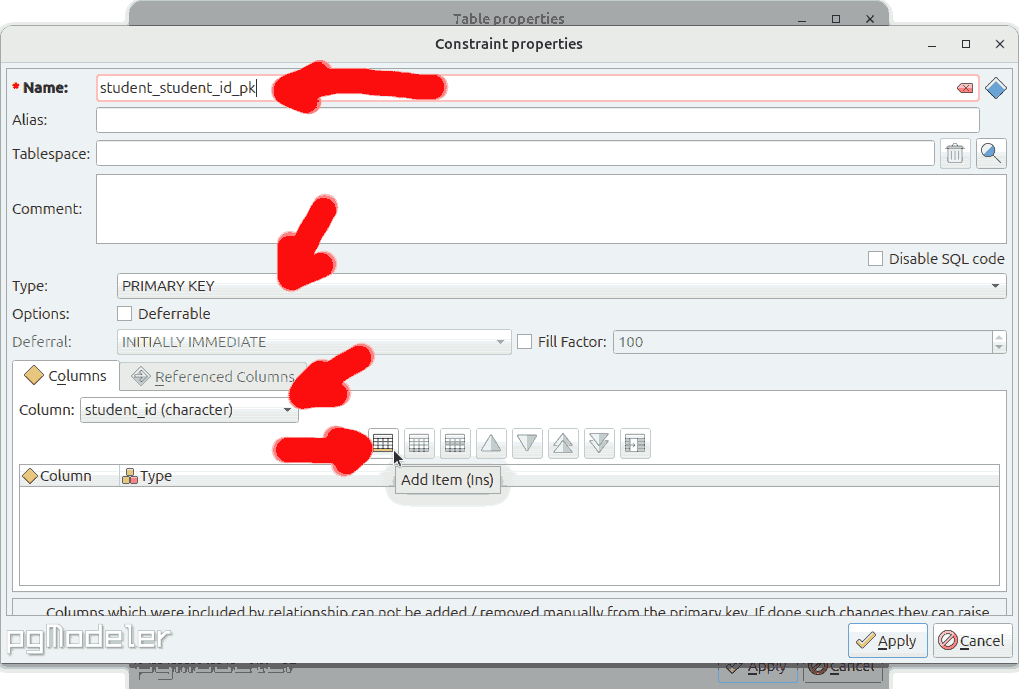
\includegraphics[width=0.48\linewidth]{\currentDir/makeStudentTable22studentIdPkData}}}%
%
\floatSep%
%
\subfloat[][%
The column \sqlil{student_id} appears in the \menu{Columns} list. %
We click on~\menu{Apply}.%
\label{fig:makeStudentTable23studentIdColAddedApply}%
]{\tightbox{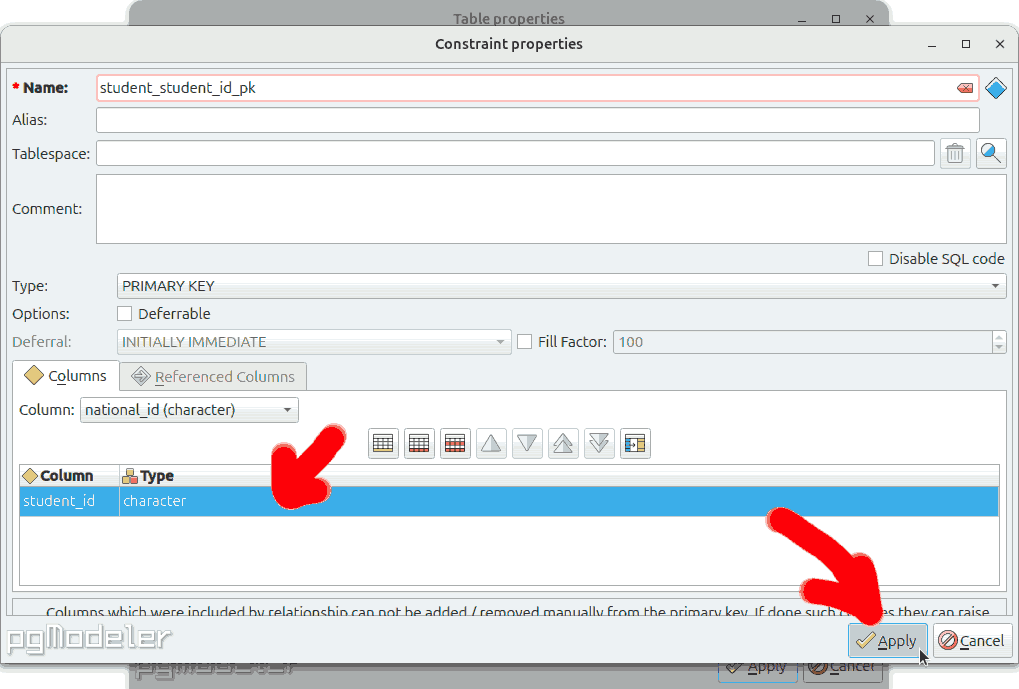
\includegraphics[width=0.48\linewidth]{\currentDir/makeStudentTable23studentIdColAddedApply}}}%
%
\floatRowSep%
%
\subfloat[][%
The new constraint appears and we click on \menu{Add Item}~\pgmodelerAddItem.%
\label{fig:makeStudentTable24studentIdAddedNewConstraint}%
]{\tightbox{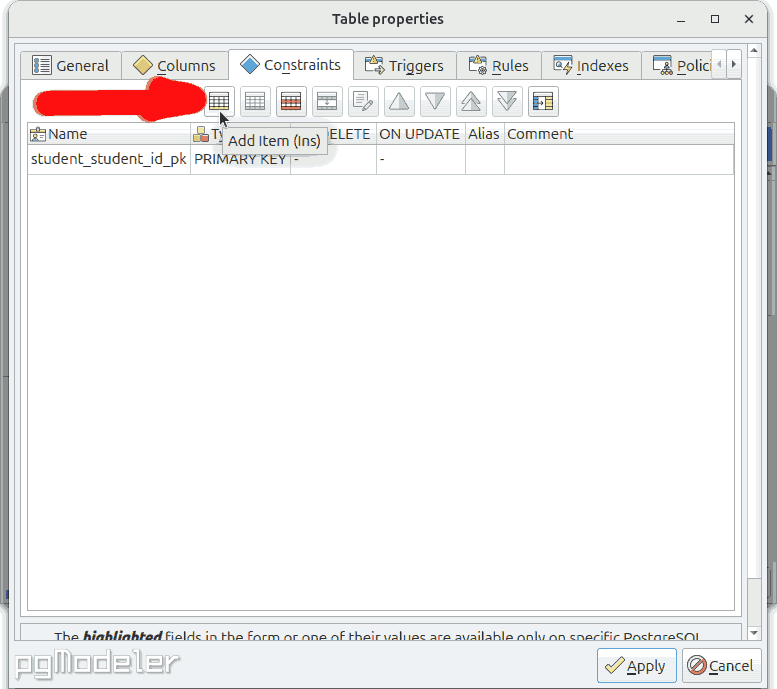
\includegraphics[width=0.48\linewidth]{\currentDir/makeStudentTable24studentIdAddedNewConstraint}}}%
%
\floatSep%
%
\subfloat[][%
We now want to add a constraint checking that the national~ID is correct. %
We call it \sqlil{student_national_id_check} and select \sqlilIdx{CHECK}\sqlIdx{CONSTRAINT!CHECK} in the \menu{Type} drop-down box.
\label{fig:makeStudentTable25nationalIdCheck}%
]{\tightbox{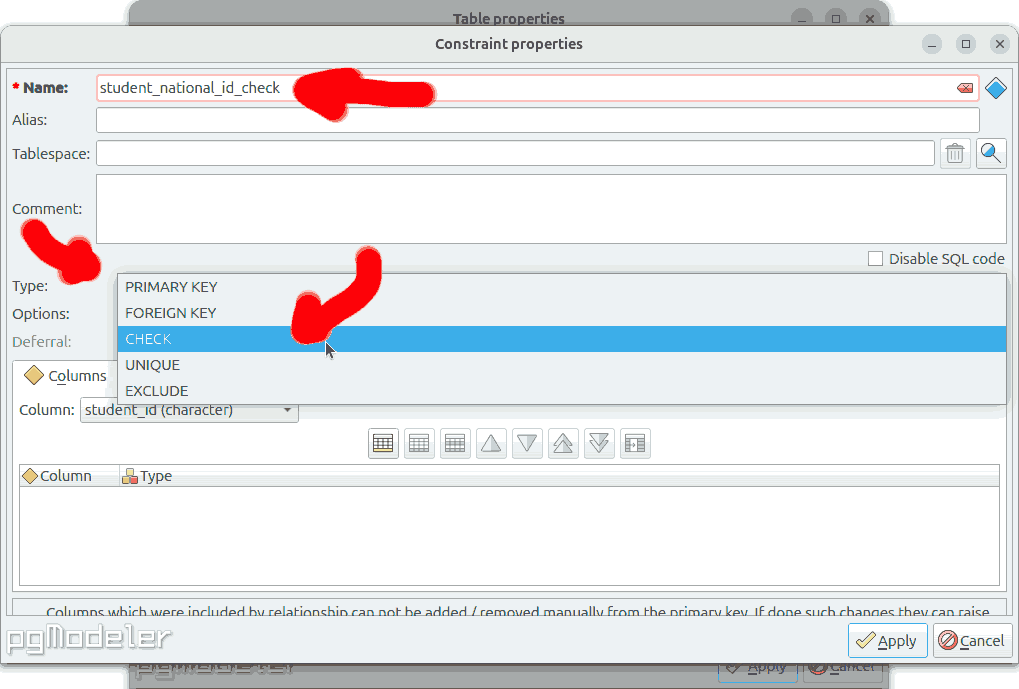
\includegraphics[width=0.48\linewidth]{\currentDir/makeStudentTable25nationalIdCheck}}}%
%
\label{fig:makeStudentTable:F}%
\caption{Developing logical models using \pgmodeler~(continued).}%
\end{figure}%
%
\begin{figure}%
\ContinuedFloat%
\centering%
%
\subfloat[][{\sloppy%
\sqlilIdx{CHECK}\sqlIdx{CONSTRAINT!CHECK} constraints are specified as \sql\ \menu{Expression}. %
To validate the field~\sqlil{national_id}, we specify the \pgls{regex} \sqlil{national_id~'^\\d\{6\}((19)|(20))\\d\{9\}[0-9X]\$'}. %
We click~\menu{Apply}.}%
\label{fig:makeStudentTable26nationalIdConstraintApply}%
]{\tightbox{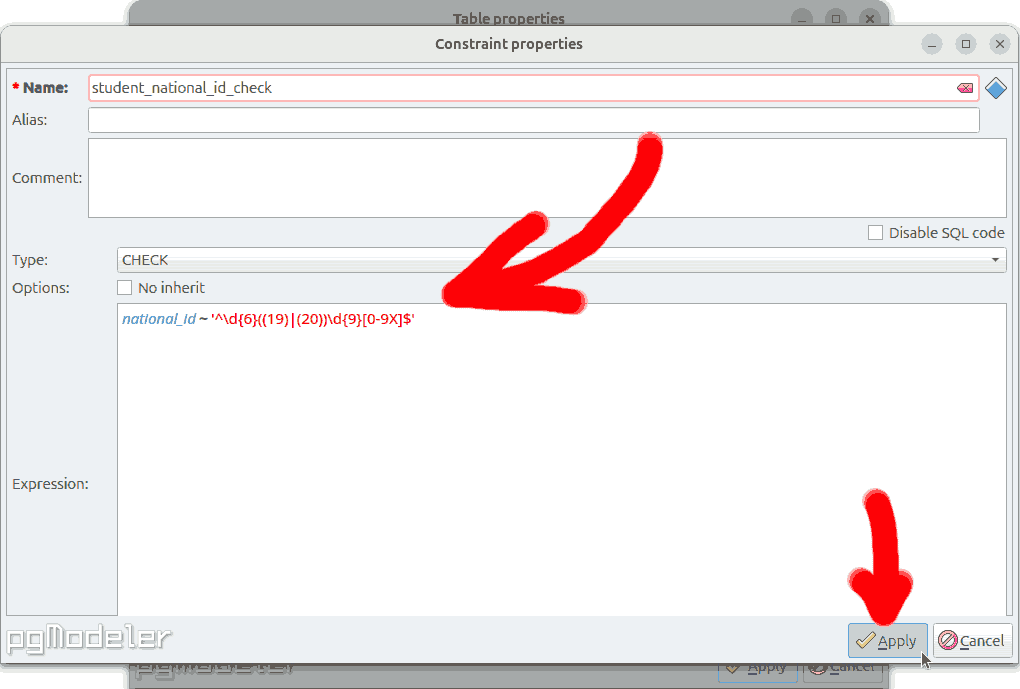
\includegraphics[width=0.48\linewidth]{\currentDir/makeStudentTable26nationalIdConstraintApply}}}%
%
\floatSep%
%
\subfloat[][%
The new constraint appears and we click on~\menu{Add Item}~\pgmodelerAddItem.%
\label{fig:makeStudentTable27nationalIdAddedNewConstraint}%
]{\tightbox{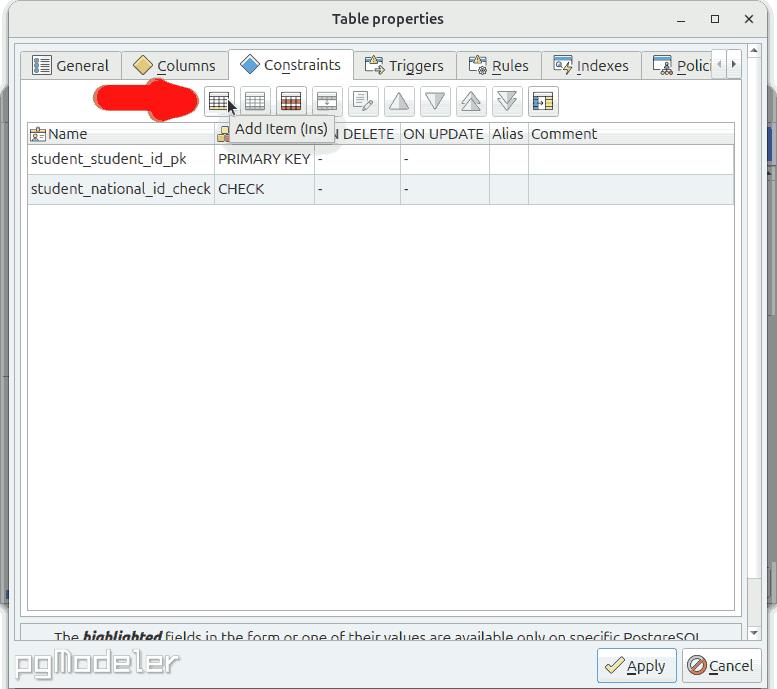
\includegraphics[width=0.48\linewidth]{\currentDir/makeStudentTable27nationalIdAddedNewConstraint}}}%
%
\floatRowSep%
%
\subfloat[][%
We create a \sqlilIdx{CHECK}\sqlIdx{CONSTRAINT!CHECK}~constraint for the column~\sqlil{mobile}. %
The expression~\sqlil{mobile ~ '^\\d\{11\}\$'} demands an 11~digit string. %
We click on~\menu{Apply}.%
\label{fig:makeStudentTable28mobileCheck}%
]{\tightbox{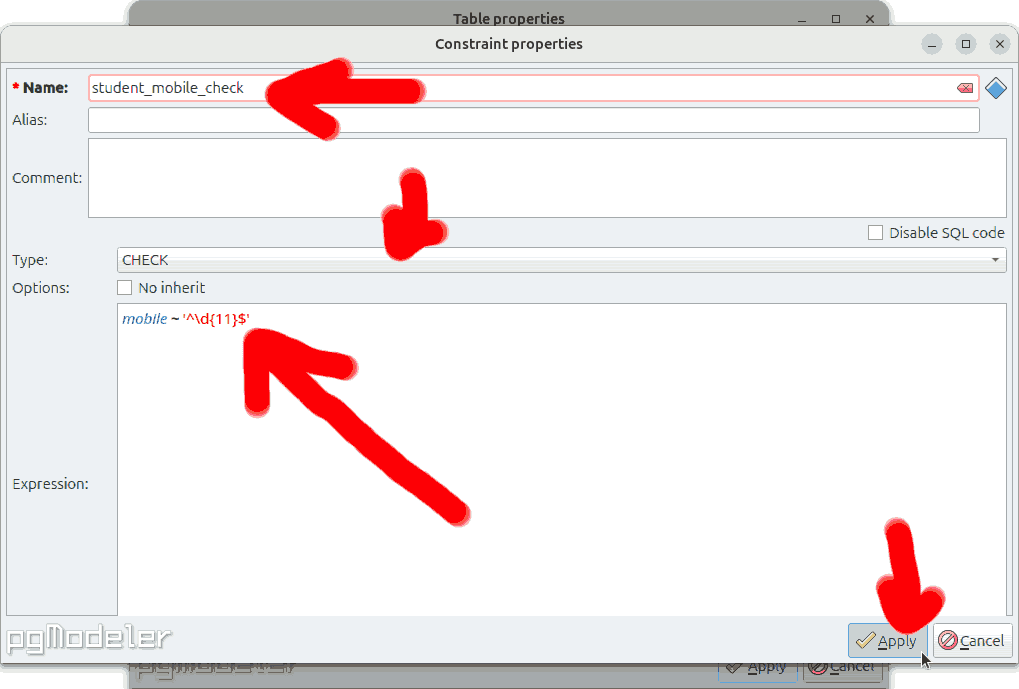
\includegraphics[width=0.48\linewidth]{\currentDir/makeStudentTable28mobileCheck}}}%
%
\floatSep%
%
\subfloat[][%
The new constraint appears and we click on~\menu{Add Item}~\pgmodelerAddItem.%
\label{fig:makeStudentTable29mobileAddedNewConstraint}%
]{\tightbox{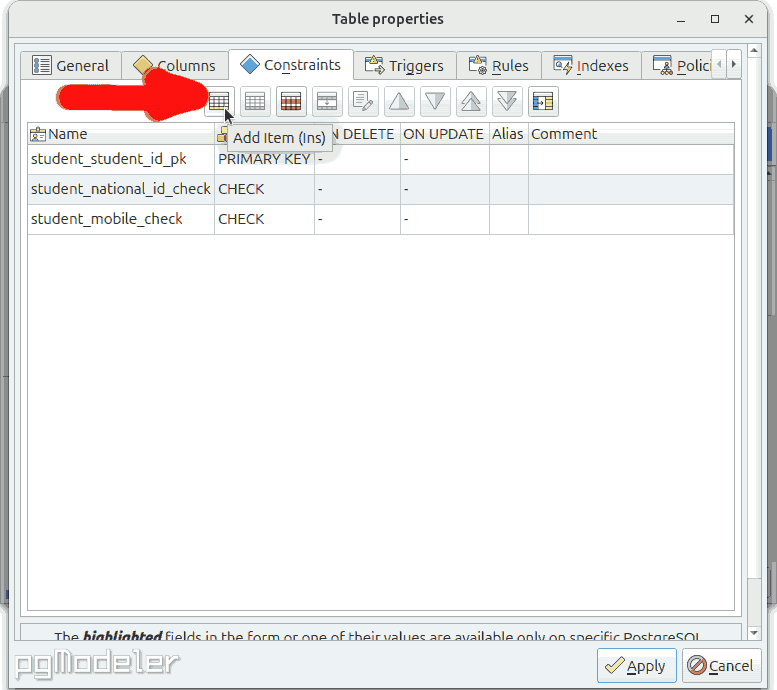
\includegraphics[width=0.48\linewidth]{\currentDir/makeStudentTable29mobileAddedNewConstraint}}}%
%
\label{fig:makeStudentTable:G}%
\caption{Developing logical models using \pgmodeler~(continued).}%
\end{figure}%
%
\begin{figure}%
\ContinuedFloat%
\centering%
%
\subfloat[][%
We specify the \sqlilIdx{CHECK}\sqlIdx{CONSTRAINT!CHECK} constraint for the \pgls{dateOfBirth} and call it~\sqlil{student_date_of_birth_check}. %
We combine the condition \sqlil{date_of_birth > '1900-01-01'}~(demanding that students may not be born before the year~1900) and \sqlil{date_of_birth < '2100-01-01'}~(which prevents students born in the 22nd century) with~\sqlilIdx{AND}. %
We click~\menu{Apply}.%
\label{fig:makeStudentTable30dateOfBirthCheck}%
]{\tightbox{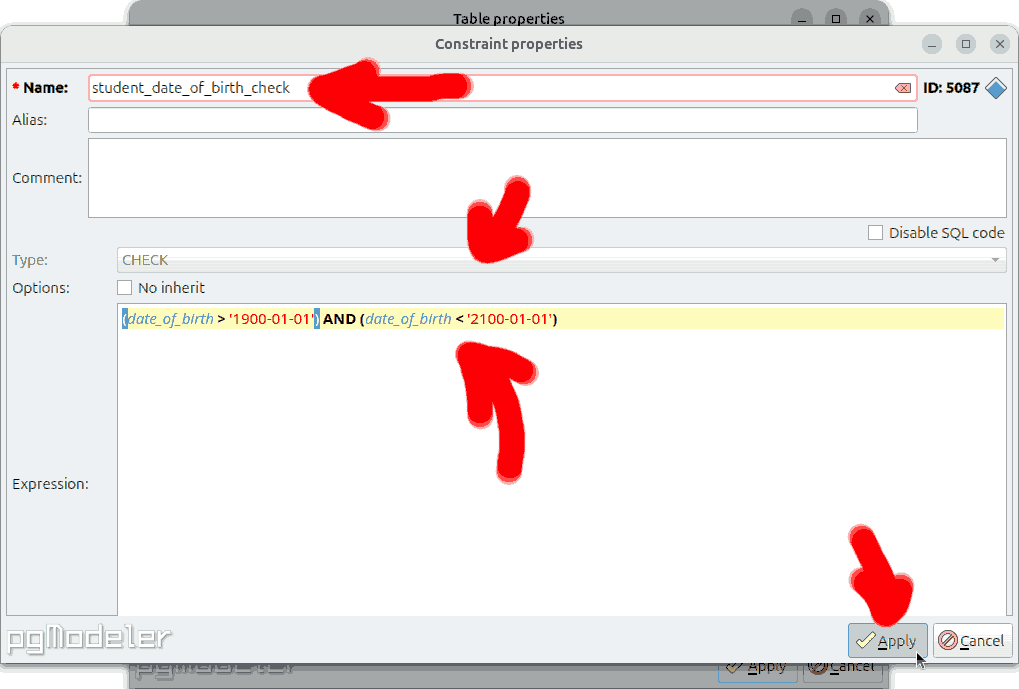
\includegraphics[width=0.48\linewidth]{\currentDir/makeStudentTable30dateOfBirthCheck}}}%
%
\floatSep%
%
\subfloat[][%
The new constraint appears and we click on~\menu{Add Item}~\pgmodelerAddItem.%
\label{fig:makeStudentTable31dateOfBirthAddedNewConstraint}%
]{\tightbox{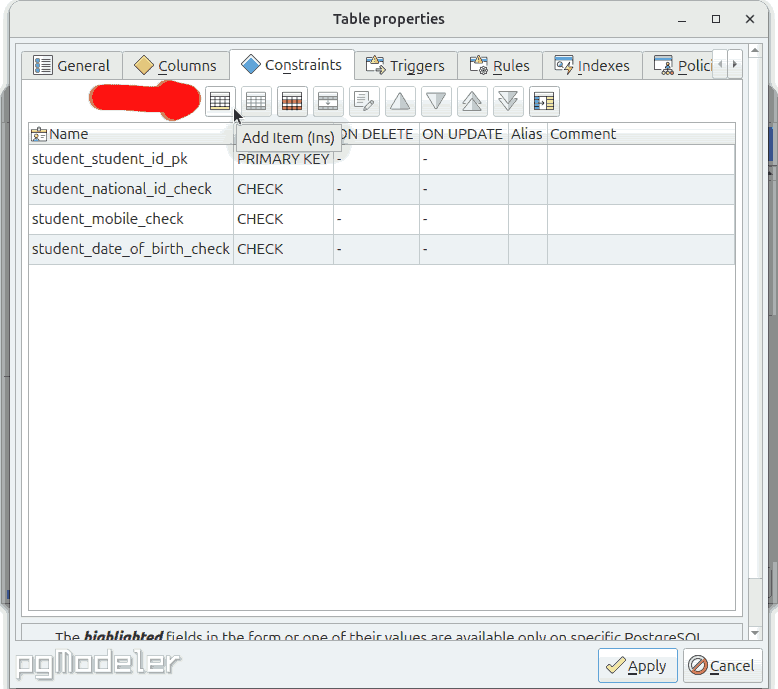
\includegraphics[width=0.48\linewidth]{\currentDir/makeStudentTable31dateOfBirthAddedNewConstraint}}}%
%
\floatRowSep%
%
\subfloat[][%
We create a \sqlilIdx{CHECK}\sqlIdx{CONSTRAINT!CHECK}~constraint for the column~\sqlil{name} and call it~\sqlil{student_name_check}. %
The expression~\expandafter\sqlil{name ~ '^\\S+.*\\S+\$'} demands that names both start and end with printable characters and may contain an arbitrary number of characters in between %
We click on~\menu{Apply}.%
\label{fig:makeStudentTable32nameCheck}%
]{\tightbox{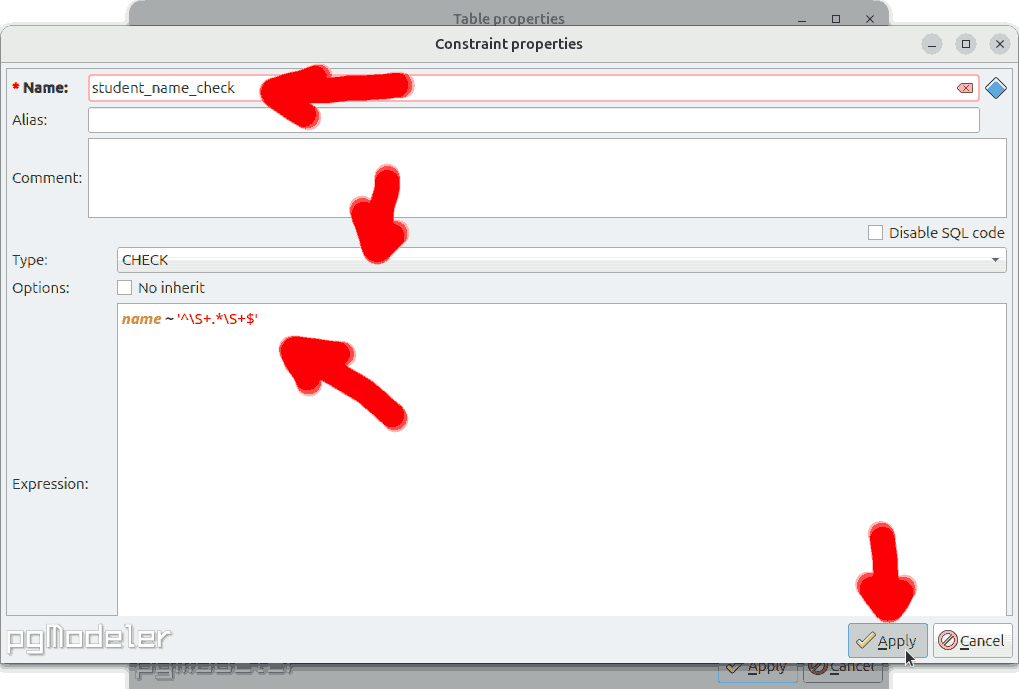
\includegraphics[width=0.48\linewidth]{\currentDir/makeStudentTable32nameCheck}}}%
%
\floatSep%
%
\subfloat[][%
The new constraint appears. %
We stop here and create the table model by clicking on~\menu{Apply}.%
\label{fig:makeStudentTable33nameCheckAddedApply}%
]{\tightbox{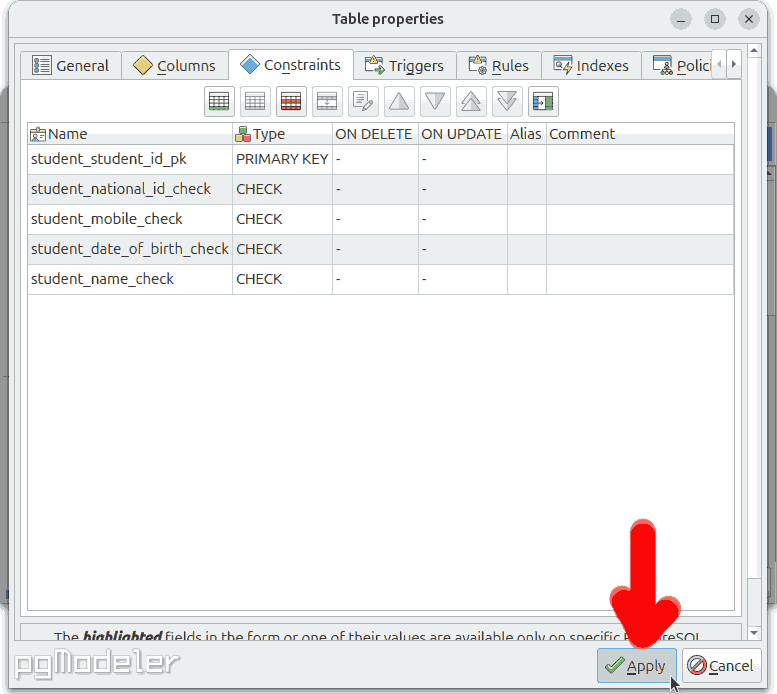
\includegraphics[width=0.48\linewidth]{\currentDir/makeStudentTable33nameCheckAddedApply}}}%
%
\label{fig:makeStudentTable:H}%
\caption{Developing logical models using \pgmodeler~(continued).}%
\end{figure}%
%
\begin{figure}%
\ContinuedFloat%
\centering%
%
\subfloat[][%
The new table appears in our \pgls{ERD}, with a syntax similar to what we had in \cref{sec:compactCrowsFootNotation}. %
We click on the main menu~\pgmodelerMainMenu.
\label{fig:makeStudentTable34modelMenu}%
]{\tightbox{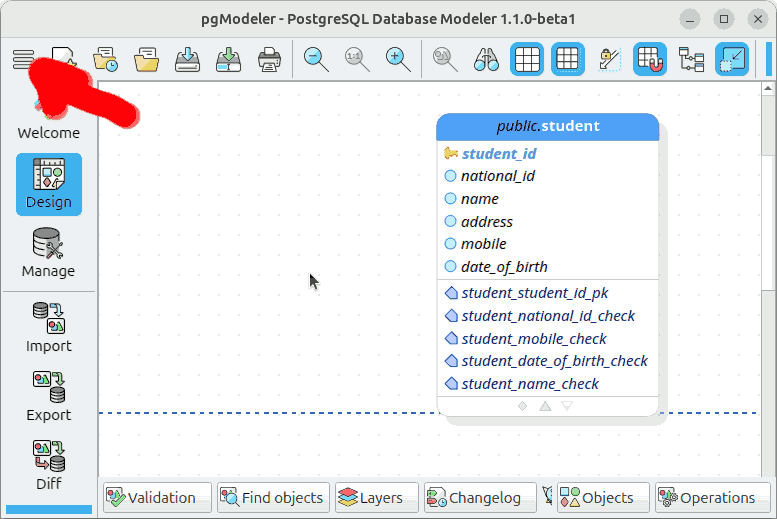
\includegraphics[width=0.48\linewidth]{\currentDir/makeStudentTable34modelMenu}}}%
%
\floatSep%
%
\subfloat[][%
It is time to save the model to a file. %
We click on~\menu{\pgmodelerMainMenu>File>Save as}.
\label{fig:makeStudentTable35saveAs}%
]{\tightbox{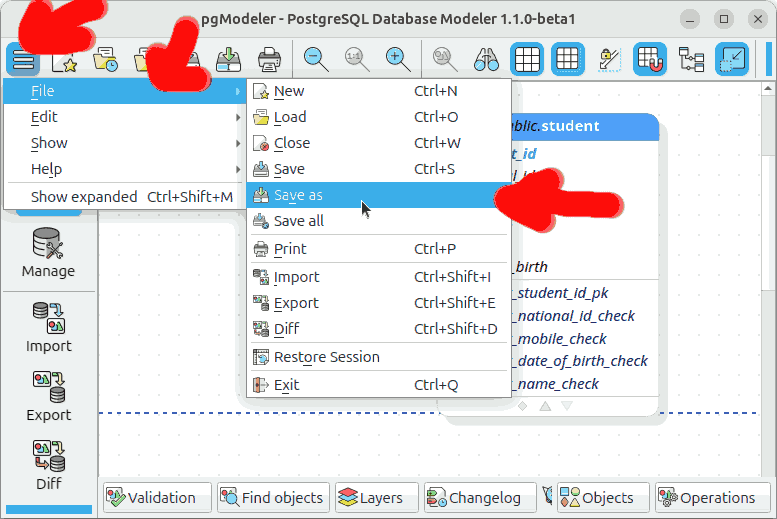
\includegraphics[width=0.48\linewidth]{\currentDir/makeStudentTable35saveAs}}}%
%
\floatRowSep%
%
\subfloat[][%
Since our model is new and unchecked~(or changed), we get asked to validate it. %
Heck, why not, we click on~\menu{Validate}.%
\label{fig:makeStudentTable36shouldValidate}%
]{\tightbox{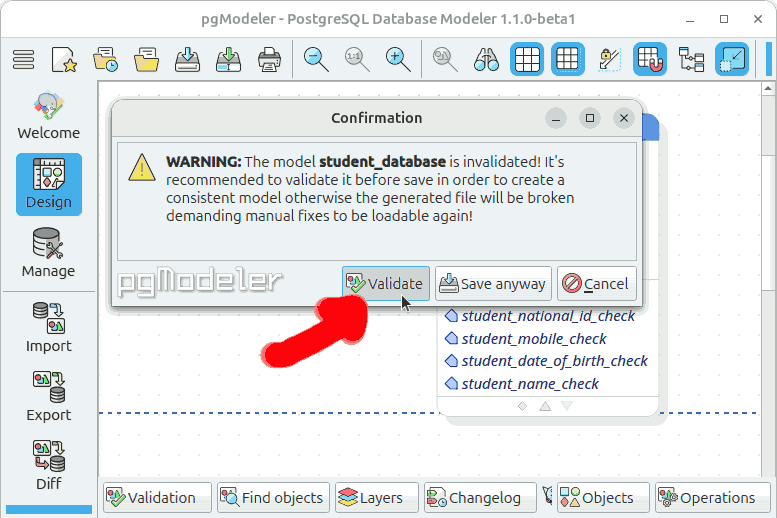
\includegraphics[width=0.48\linewidth]{\currentDir/makeStudentTable36shouldValidate}}}%
%
\floatSep%
%
\subfloat[][%
We can now select a file name and directory where the model should be stored. %
We choose the name \sqlil{student_database_1} and click~\menu{Save}.%
\label{fig:makeStudentTable37saveAsWhere}%
]{\tightbox{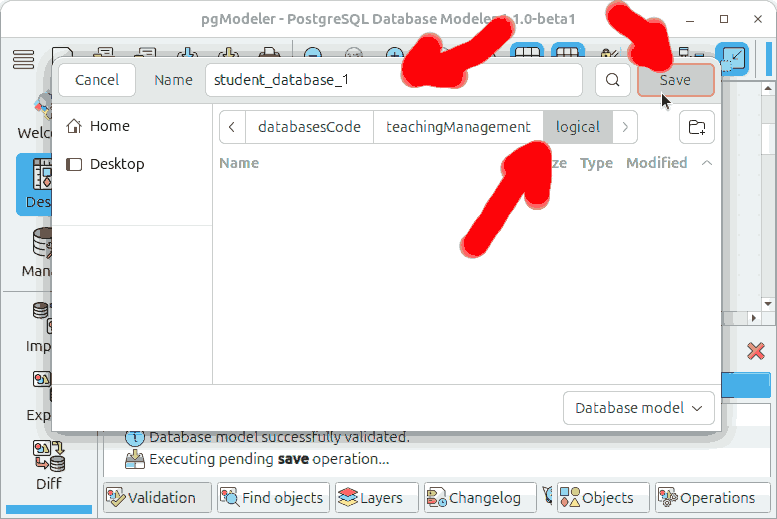
\includegraphics[width=0.48\linewidth]{\currentDir/makeStudentTable37saveAsWhere}}}%
%
\label{fig:makeStudentTable:I}%
\caption{Developing logical models using \pgmodeler~(continued).}%
\end{figure}%
%
\begin{figure}%
\ContinuedFloat%
\centering%
%
\subfloat[][%
This takes us back to the main window. %
We notice a bar with new buttons, including one called~\menu{Validate}. %
We click on it.%
\label{fig:makeStudentTable38validate}%
]{\tightbox{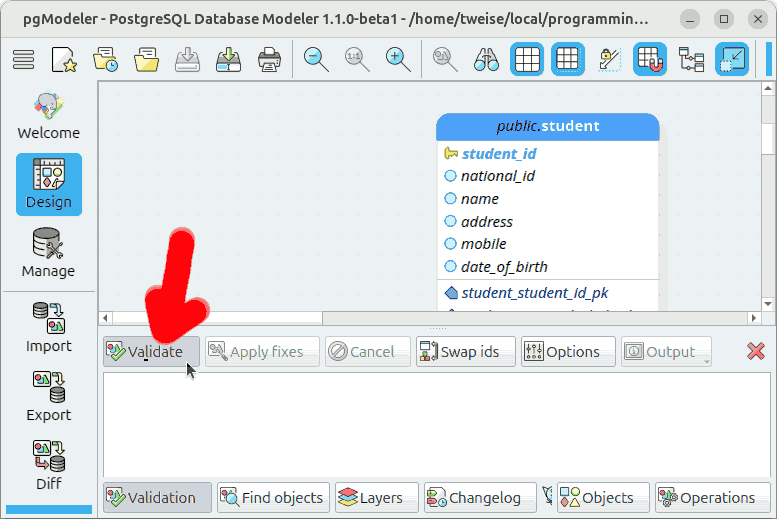
\includegraphics[width=0.48\linewidth]{\currentDir/makeStudentTable38validate}}}%
%
\floatSep%
%
\subfloat[][%
Our model gets validated. %
It is OK. %
We can close the log.%
\label{fig:makeStudentTable39validated}%
]{\tightbox{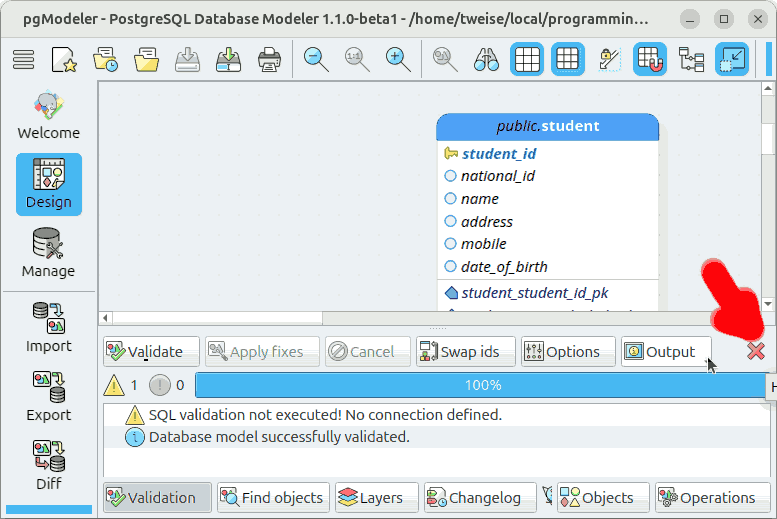
\includegraphics[width=0.48\linewidth]{\currentDir/makeStudentTable39validated}}}%
%
\floatRowSep%
%
\subfloat[][%
We now want to export the model and, thus, click on~\menu{Export}.%
\label{fig:makeStudentTable40export}%
]{\tightbox{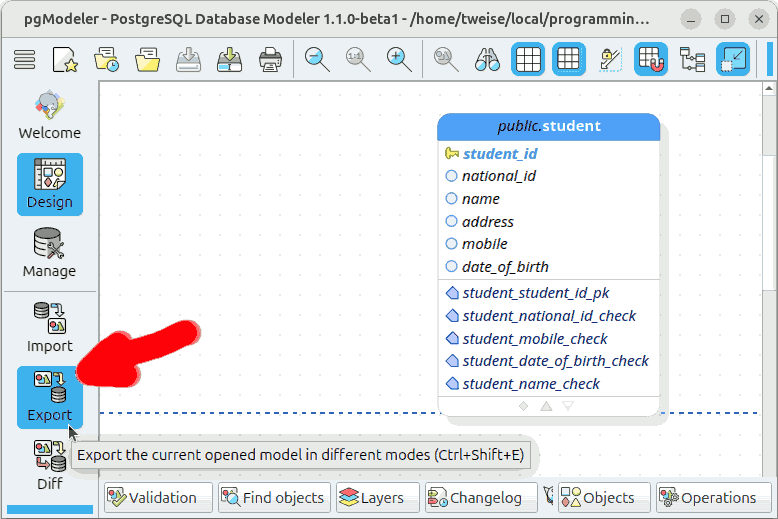
\includegraphics[width=0.48\linewidth]{\currentDir/makeStudentTable40export}}}%
%
\floatSep%
%
\subfloat[][%
We want to store it as graphic. %
So we click on \menu{Graphics file} and select \menu{Vectorial~(SVG)}, which will store the model in \pgls{SVG}~format. %
We then click into the \menu{File}~bar.
\label{fig:makeStudentTable41exportAsSvg}%
]{\tightbox{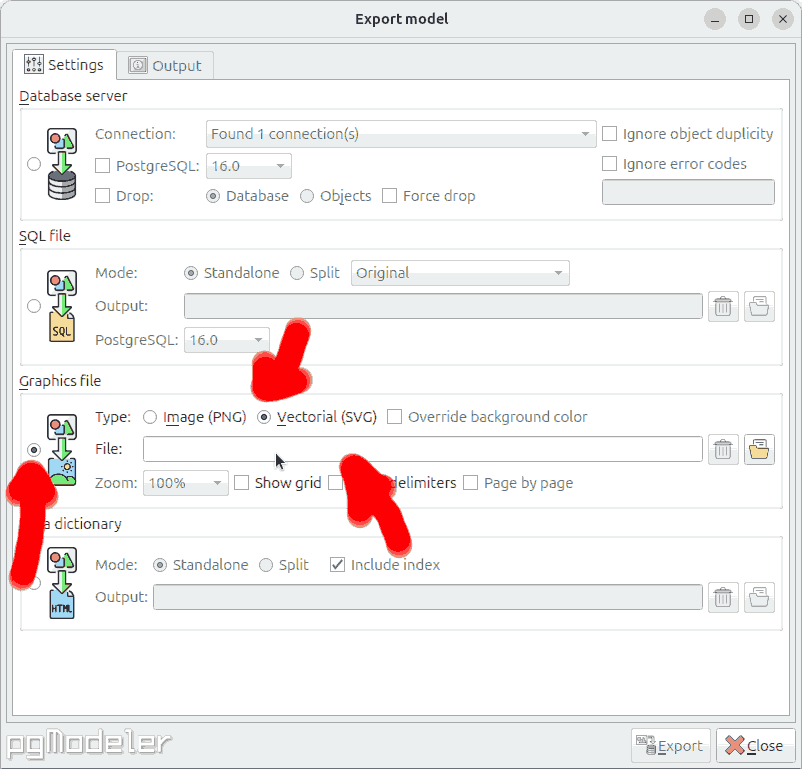
\includegraphics[width=0.48\linewidth]{\currentDir/makeStudentTable41exportAsSvg}}}%
%
\label{fig:makeStudentTable:J}%
\caption{Developing logical models using \pgmodeler~(continued).}%
\end{figure}%
%
\begin{figure}%
\ContinuedFloat%
\centering%
%
\subfloat[][%
We again get to select a file name and stick with \sqlil{student_database_1}. %
We click on~\menu{Save}.%
\label{fig:makeStudentTable42fileName}%
]{\tightbox{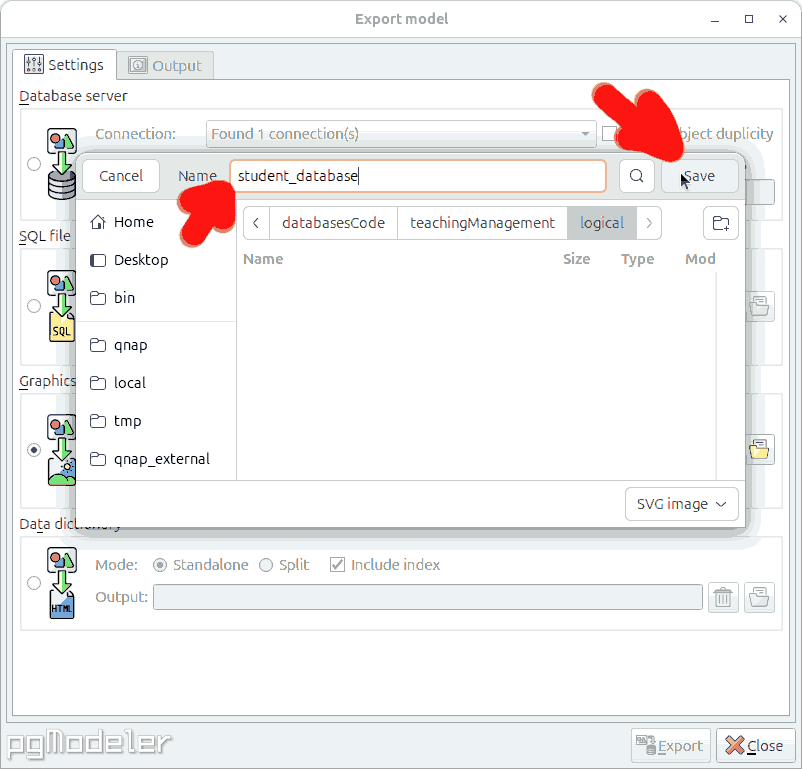
\includegraphics[width=0.48\linewidth]{\currentDir/makeStudentTable42fileName}}}%
%
\floatSep%
%
\subfloat[][%
We can now click on~\menu{Export}.%
\label{fig:makeStudentTable43exportToSvgExport}%
]{\tightbox{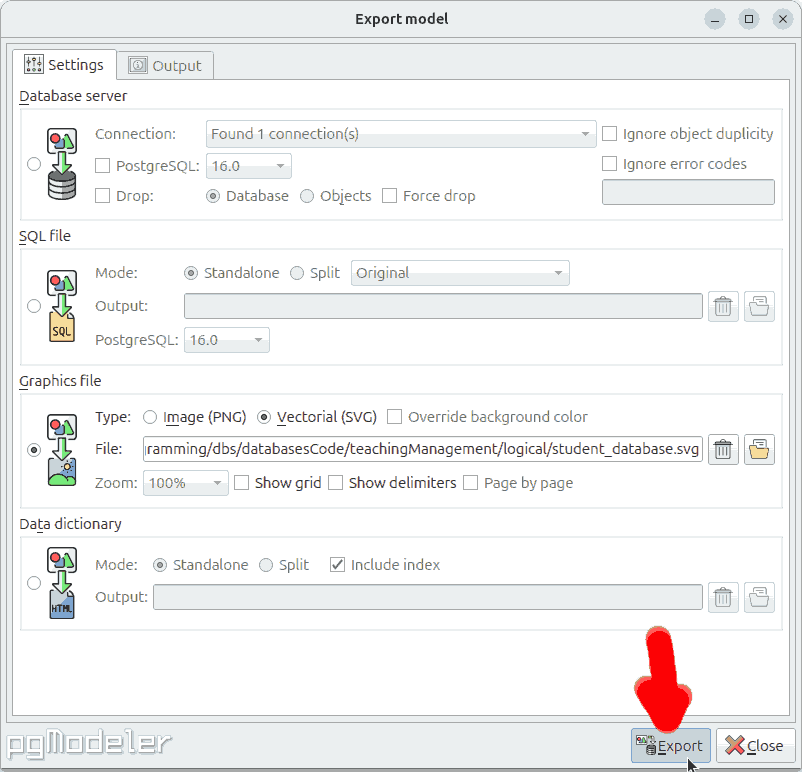
\includegraphics[width=0.48\linewidth]{\currentDir/makeStudentTable43exportToSvgExport}}}%
%
\floatRowSep%
%
\subfloat[][%
The file has been exported, we can close the dialog.%
\label{fig:makeStudentTable44exportToSvgExported}%
]{\tightbox{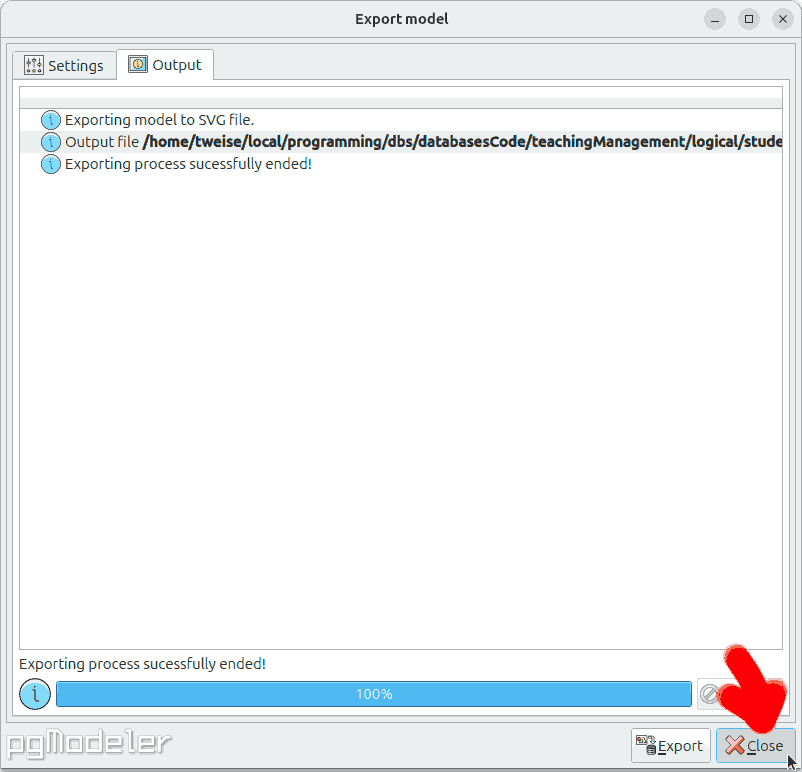
\includegraphics[width=0.48\linewidth]{\currentDir/makeStudentTable44exportToSvgExported}}}%
%
\floatSep%
%
\subfloat[][%
This is the exported vector graphic. %
It looks quite nice. %
If we had done a bigger model with many tables, it would probably look quite exciting.%
\label{fig:makeStudentTable45svg}%
]{\parbox[t]{0.48\linewidth}{\centering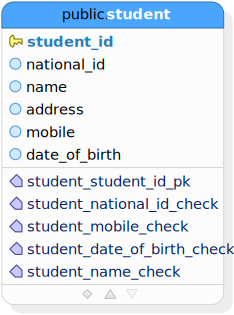
\includegraphics[width=0.66\linewidth]{\currentDir/makeStudentTable45svg}}}%
%
\label{fig:makeStudentTable:K}%
\caption{Developing logical models using \pgmodeler~(continued).}%
\end{figure}%
%
\begin{figure}%
\ContinuedFloat%
\centering%
%
\subfloat[][%
We open the \menu{Export} dialog again. %
This time, we want to export our model to~\sql. %
We click on~\menu{SQL file}. %
\textcolor{red}{Important:~Mark the output as \emph{Split}.} %
Then on the file bar.%
\label{fig:makeStudentTable46exportToSql}%
]{\tightbox{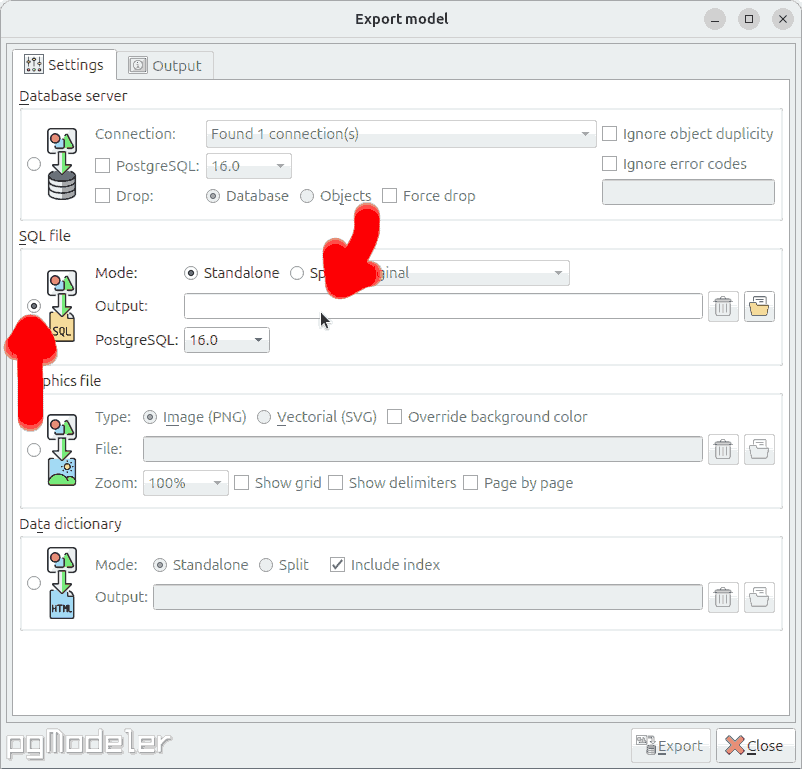
\includegraphics[width=0.48\linewidth]{\currentDir/makeStudentTable46exportToSql}}}%
%
\floatSep%
%
\subfloat[][%
Because we want to output the model using the \emph{split} method, this will create multiple \sql~files. %
Instead of a file name, we need to choose a folder name. %
We therefore create a new folder and choose~\sqlil{generated_sql} as its name. %
\label{fig:makeStudentTable47folderName}%
]{\tightbox{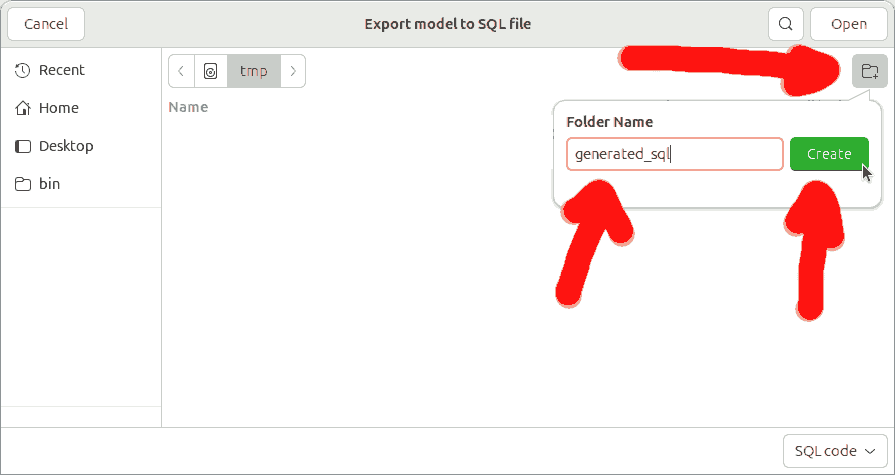
\includegraphics[width=0.48\linewidth]{\currentDir/makeStudentTable47folderName}}}%
%
\floatRowSep%
%
\subfloat[][%
The folder is created, we click on~\menu{Open}.%
\label{fig:makeStudentTable48folderOpen}%
]{\tightbox{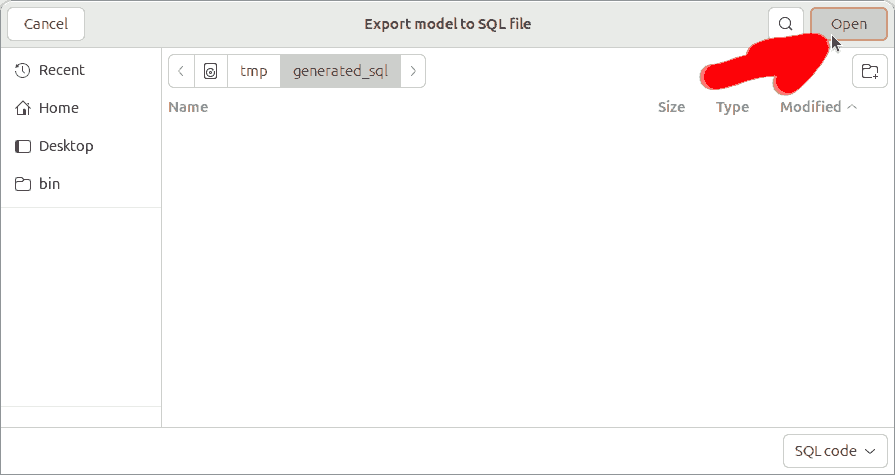
\includegraphics[width=0.48\linewidth]{\currentDir/makeStudentTable48folderOpen}}}%
%
\floatSep%
%
\subfloat[][%
This takes us back to the \emph{Export model} dialog, where we click on~\menu{Export}.%
\label{fig:makeStudentTable49export}%
]{\tightbox{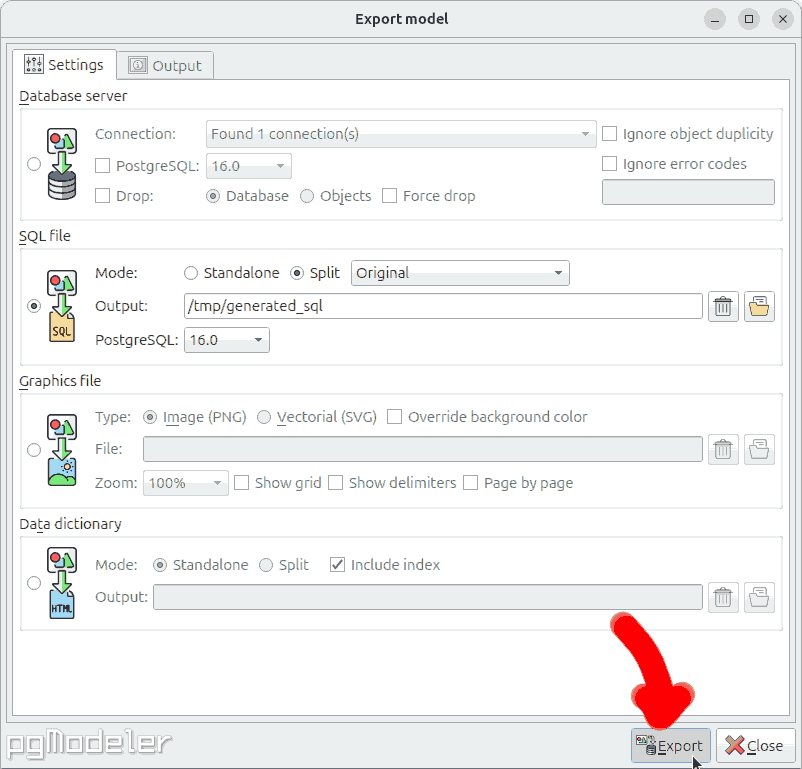
\includegraphics[width=0.48\linewidth]{\currentDir/makeStudentTable49export}}}%
%
\label{fig:makeStudentTable:L}%
\caption{Developing logical models using \pgmodeler~(continued).}%
\end{figure}%
%
\begin{figure}%
\ContinuedFloat%
\centering%
%
\subfloat[][%
The logical model is exported to \sql. %
We can close the dialog by clicking on~\menu{Close}.%
\label{fig:makeStudentTable50exported}%
]{\tightbox{\includegraphics[width=0.48\linewidth]{\currentDir/makeStudentTable50exported}}}%
%
\floatSep%
%
\subfloat[][%
We can browse to the folder using whatever file browser the \pgls{OS} offers. %
We find that it contains several files, whose contents are shown in \cref{lst:logical:teachingManagment:student_database_1:01_student_database_database_2001,lst:logical:teachingManagment:student_database_1:03_public_student_table_5071}. %
We can execute them on the \postgresql\ \pgls{server} using \psql. %
We do this in \cref{exec:logical:teachingManagment:student_database_1:01_student_database_database_2001,exec:logical:teachingManagment:student_database_1:03_public_student_table_5071}.%
\label{fig:makeStudentTable51explorer}%
]{\tightbox{\includegraphics[width=0.48\linewidth]{\currentDir/makeStudentTable51explorer}}}%
%
\label{fig:makeStudentTable:M}%
\caption{Developing logical models using \pgmodeler~(continued).}%
\end{figure}%
%
\gitSQLAndOutput{\databasesCodeRepo}{teachingManagement/logical/student_database_1/generated_sql}{01_student_database_database_2001.sql}{}{}{}{postgres.sh}{logical:teachingManagment:student_database_1:01_student_database_database_2001}{%
This auto-generated \sql\ script creates the \db~\sqlil{student_database}.%
}%
%
\gitSQLAndOutput{\databasesCodeRepo}{teachingManagement/logical/student_database_1/generated_sql}{03_public_student_table_5071.sql}{student_database}{}{}{postgres.sh}{logical:teachingManagment:student_database_1:03_public_student_table_5071}{%
This auto-generated \sql\ script creates the table~\sqlil{student} inside the \db~\sqlil{student_database}.%
}%
%
\gitSQLAndOutput{\databasesCodeRepo}{teachingManagement/logical/student_database_1}{insert.sql}{student_database}{}{}{postgres.sh}{logical:teachingManagment:student_database_1:insert}{%
We can insert some records into the table~\sqlil{student}.%
}%
%
\gitSQLAndOutput{\databasesCodeRepo}{teachingManagement/logical/student_database_1}{cleanup.sql}{}{}{}{postgres.sh}{logical:teachingManagement:student_database_1:cleanup}{%
Cleaning up after the student \db\ example.%
}%
%
%
Back when we just began discussing conceptual models, we tried to model the entity type~\emph{Student}.
We drew an \pgls{ERD} for students as~\cref{fig:yedErdEntitiesA21erd}, which I here reproduce as \cref{fig:yedErdEntitiesA21erd2}.
Here, each entity of type \emph{Student} will have a name, an~ID, a student\nobreakdashes-ID, an address, a mobile phone number, and a \glsreset{dateOfBirth}\pgls{dateOfBirth}.
Later on, we realized that this model has many shortcomings and is not suitable for our teaching management platform.
Yet, it is fairly simple and suitable as an example for translating a single entity type from the conceptual model to the logical model.

We want to use the \pgmodeler\ for doing so.
Under \ubuntu\ \linux, we can start this program by opening a \pgls{terminal} by hitting \ubuntuTerminal, typing in \bashil{pgmodler}, and hitting~\keys{\enter}, as shown in \cref{fig:makeStudentTable01startPgmodeler}.
Under \microsoftWindows, you would instead proceed as shown in \cref{fig:installingPgModelerWindows22pgmodelerLogo}.

In the opened \pgmodeler\ window, we click on \menu{New Model} in \cref{fig:makeStudentTable02newModel}.
An empty \pgls{ERD} opens that represents an (empty) \db.
In a first step, we should choose a proper name for our \db.
We right-click at some place in the empty \pgls{ERD}.
In the context menu that opens up, we click on~\menu{Properties}, as shown in \cref{fig:makeStudentTable03rightClickProperties}.
A dialog called \inQuotes{Database Properties} opens.
As said, we want to set a proper name for our new \db.
We choose \sqlil{student_database} -- because the \db\ will only have a single table named \sqlil{student} -- and then click on~\menu{Apply} in \cref{fig:makeStudentTable04propertiesNameApply}.

Back in the \pgls{ERD} view it is now time for creating the table that will represent our \emph{Student} entity type.
We therefore again right-click into the (empty) diagram.
In the popup-menu, we click on~\menu{New>Schema Object>Table}, as illustrated in \cref{fig:makeStudentTable05newTable}.

The \inQuotes{Table properties} dialog opens in \cref{fig:makeStudentTable06tableNameColumns}.
We can choose a table name and, as said, we pick \sqlil{student} and type this in.
The attributes of an entity type become attributes in a relation in a relational logical schema, which are embodied as columns of a table.
To add such columns, we click on the register~\menu{Columns}.
The columns register is still empty.
We click on the \menu{Add Item} symbol~\pgmodelerAddItem\ in \cref{fig:makeStudentTable07newColumn}.

In a first step, we want to create a column for the university-issued student~ID.
As name for this column, we choose~\sqlil{student_id}.
This is better than using~\sqlil{ID}, because it conveys a clear meaning that this is, in fact, the student~ID.
Everybody will immediately understand what this means.
Student~IDs are usually strings of a fixed length.
We therefore choose the \menu{Type}~\sqlil{character}\sqlIdx{CHARACTER} in \cref{fig:makeStudentTable08studentIdNameAndType}.
In \sql, this is the datatype for fixed-length strings.
As (fixed) length, we enter~11 in the \menu{L:}~field.
This means that all student~IDs that we store in our \db\ will be text strings consisting of eleven characters.
We also mark the column as \sqlilIdx{NOT NULL}.
This means that there cannot be a student record where the \sqlil{student_id} is \sqlilIdx{NULL}.
This, in turn, means that there cannot be a student record without student~ID.
\sqlil{student_id} is a mandatory field that always needs to be provided.
In \cref{fig:makeStudentTable09studentIdLenNotNullApply}, we click~\menu{Apply}.%
%
\bestPractice{columnNames}{%
To avoid issues with quotations, it is best to use only lower case character names and underscores~(\sqlil{_}) to separate words for all named things in \pgmodeler, including tables, columns, and constraints.%
}%
%
The new column appears in the table creation dialog.
We now want to add the next column, so we click again on~\menu{Add Item}~\pgmodelerAddItem\ in \cref{fig:makeStudentTable10studentIdAddedNewColumn}.
The next important piece of data of each student record is a national Chinese~ID number~(中国公民身份号码).
We add the column \sqlil{national_id} for storing Chinese~ID numbers.
As per standard \mbox{GB11643\nobreakdashes-1999} \citetitle{GB116431999CIN}~\cite{GB116431999CIN}, such numbers always consist of 18~characters.
So we choose the atatype \sqlil{character}\sqlIdx{CHARACTER} with the fixed length~18.
We here ignore the fact that there could be foreign exchange students~(留学生) and demand that all records must have \sqlil{national_id} field set by marking the column as~\sqlilIdx{NOT NULL}.
We click~\menu{Apply} in \cref{fig:makeStudentTable11nationalIdNameTypeLenNotNullApply}.

The new column appears in \cref{fig:makeStudentTable12nationalIdAddedNewColumn} and we click~\menu{Add Item}~\pgmodelerAddItem.
We now define the column \sqlil{name} for student names.
Names are text strings of variable length, which corresponds to the \sql\ datatype \sqlil{varchar}\sqlIdx{VARCHAR}.
We set the \emph{maximum} length to 255~characters, which is fairly large and should be long enough for most sensible names.
Each student must have a name, so we again specify \sqlil{NOT NULL} and click~\menu{Apply} in \cref{fig:makeStudentTable13nameNameTypeLenNotNullApply}.

The new column appears in \cref{fig:makeStudentTable14nameAddedNewColumn} and we click again on~\menu{Add Item}~\pgmodelerAddItem.
The next column we want to add is for storing the addresses of the students.
We call this column \sqlil{address}.
Here, we again use strings of variable length~(type \sqlil{varchar}\sqlIdx{VARCHAR}) as datatype.
We again set the maximum length to 255~characters.
We also again require the field to be \sqlilIdx{NOT NULL} and click~\menu{Apply} in \cref{fig:makeStudentTable15addressNameTypeLenNotNullApply}.

The new column appears in \cref{fig:makeStudentTable16addressAddedNewColumn} and we click~\menu{Add Item}~\pgmodelerAddItem.
We now add a column for \sqlil{mobile} phone numbers.
Mobile phone numbers in China have 11~digits~\cite{BD2006BDBK:MPNANSBTTMDFMP}.
We can thus store them as strings~~(\sqlil{character}\sqlIdx{CHARACTER}) of the fixed length~11.
We require that they must be specified~(\sqlilIdx{NOT NULL}) and click~\menu{Apply} in \cref{fig:makeStudentTable17mobileNameTypeLenNotNullApply}.

The new column appears in the table dialog and we again click on~\menu{Add Item}~\pgmodelerAddItem\ in \cref{fig:makeStudentTable18mobileAddedNewColumn}.
Finally, we add the \pgls{dateOfBirth} in form of the \sqlil{date_of_birth} column.
The datatype here is \sqlil{date}\sqlIdx{DATE}.
Like all the columns so far, we require that \pglspl{dateOfBirth} to be \sqlilIdx{NOT NULL}.
We click~\menu{Apply} in \cref{fig:makeStudentTable19dateOfBirthNameTypeNotNullApply}.

The new column appears in~\cref{fig:makeStudentTable20dateOfBirthAddedConstraints}.
In the above text, you may have noticed that we are quite lenient with the data.
For example, mobile phone numbers are not strings of arbitrary characters, but consist only of digits.
Chinese ID~numbers also are composed of digits, with the exception that the last character might be an~\textil{X}.
Also, we should probably not permit arbitrary dates as \pglspl{dateOfBirth}.
Even though September~23,~1811 would be a totally valid date, as the \pgls{dateOfBirth} of a student it would be unusual.
Actually, we already learned how to deal with such restrictions on valid data back in \dref{sec:factory:table:customer}:
by using constraints.
We also did not yet define a primary key~(see \cref{def:primaryKey}) for our table.

We click on the register \menu{Constraints}, because now we want to add validity rules for our data.
In the \menu{Constraints} register, we click~\menu{Add Item}~\pgmodelerAddItem, as shown in \cref{fig:makeStudentTable21newConstraint}.
If you think about, we can consider the fact that a column is the \emph{primary key} as a combination of a \sqlilIdx{UNIQUE} and a \sqlilIdx{NOT NULL} constraint~(maybe together with some special indexing for fast access).
So first, we want to choose a primary key.

What would be the most suitable column for use as primary key?
The columns \sqlil{name}, \sqlil{address}, and \sqlil{date_of_birth} are unsuitable -- if not for obvious reasons -- then at least because they are not necessarily unique.
The two columns \sqlil{student_id} and \sqlil{national_id} both look promising a primary keys.
However, a person may enroll several times, maybe first as Bachelor and later as Master's student.
Hence, \sqlil{national_id} is not necessarily unique.
But for each enrollment, the person gets a new \sqlil{student_id}, which therefore is unique.
As first constraint, we thus want to define \sqlil{student_id} as the primary key of our table.

We call this constraint \sqlil{student_student_id_pk} and select \sqlilIdx{PRIMARY KEY} as type.
We select the column \sqlil{student_id} in the \menu{Column} drop-down box and click on~\menu{Add Item}~\pgmodelerAddItem\ in \cref{fig:makeStudentTable22studentIdPkData}.
The column \sqlil{student_id} appears in the \menu{Columns} list.
We click on~\menu{Apply} in \cref{fig:makeStudentTable23studentIdColAddedApply}.%
%
\bestPractice{constraintNames}{%
Constraints should have descriptive names~\cite{B2025DS:SBPASG}. %
If some table modification fails, we will see the name of the constraint that was violated. %
If the name makes sense and is easy to understand, then this makes it easier to find out what went wrong and why.%
}%
%
The new constraint appears and we click on \menu{Add Item}~\pgmodelerAddItem\ in \cref{fig:makeStudentTable24studentIdAddedNewConstraint}.
We now want to add a constraint checking that the national~ID is correct.
We call it \sqlil{student_national_id_check} and select \sqlilIdx{CHECK}\sqlIdx{CONSTRAINT!CHECK} in the \menu{Type} drop-down box in \cref{fig:makeStudentTable25nationalIdCheck}.
Indeed, we are going to create a \sqlil{CHECK} constraint\sqlIdx{CONSTRAINT!CHECK}.
For this, we just need to provide an \sql\ \menu{Expression}.
This expression is evaluated whenever a row is added to the table or when a row is changed.
If it then returns~\sqlil{TRUE}, everything is fine.
If it returns~\sqlil{FALSE}, then the change will not be made.

So back to the Chinese~ID numbers~(中国公民身份号码).
How do we check them?
Standard \mbox{GB11643\nobreakdashes-1999} \citetitle{GB116431999CIN}~\cite{GB116431999CIN} tells us that the first six digits are the administrative division code.
The next eight digits are the \pgls{dateOfBirth} in format YYYYMMDD, followed by three digits of order code.
The last character is a single checksum digit~(which can be~X).
We could check this in a super fancy fashion.
We could get our hands on a list of the actual valid values for the first digits, assuming that not all possible 1\decSep000\decSep000~possible administrative division codes are actually valid.
We could compare the next six digits to the \pgls{dateOfBirth} that we store as well\footnote{%
On second thought, if we require ID numbers to be present, we would not need to store the \pgls{dateOfBirth} anymore {\dots} but well, now we did it and will stick to it.}.
We could even try to compute the checksum digit and check whether it matches.%
%
\begin{sloppypar}%
This is all too complicated for us.
Instead, we will resort to a \glsreset{regex}\pgls{regex} to check the field like back in \dref{sec:factory:table:customer}.
We write \expandafter\sqlil{national_id ~ '^\\d\{6\}((19)|(20))\\d\{9\}[0-9X]\$'}.
The \sqlil{national_id ~ xxx} means that the value of \sqlil{national_id} must match to some \pgls{regex}~\textil{xxx}.
In the \pgls{regex}, \textil{^}~indicates the start of the text.
\textil{\\d\{6\}}~means that six digits must immediately follow~\textil{^}, i.e., be right at the start of the string.
Then comes \textil{((19)|(20))}, which means that the next two characters must be either \inQuotes{19} or \inQuotes{20}.
This is because we do not permit \pglspl{dateOfBirth} before the year 19\textcolor{gray}{00} or after 20\textcolor{gray}{99}.
After that, we require nine digits to follow via~\textil{\\d\{9\}}.
This means we now have $6+2+9=17$~digits, leaving the final checksum character, which can be any digit from 0~to~9 or~X.
This is expressed by the~\textil{[0-9X]}.
The~textil{\$} that follows marks the end of the string, which, hence, must come directly after the checksum digit.%
\end{sloppypar}%
%
You may ask:
Why do we create such a trivial constraint?
Well, this constraint would still guard against several possible typos.
Verifying the checksum with a \pgls{regex} is probably not possible anyway, at least not with a \pgls{regex} of reasonable complexity.
Eventually, we would create an application program through which the administrative staff enters student information.
This program should then check the checksum of the \sqlil{national_id} field.

So you may ask:
If we check the national~ID value in the application anyway, then why do we put a constraint here?
We could just leave it away and assume that the application will check the validity of the field.
The answer is \emph{defense in depth}.%
%
\bestPractice{defenseInDepth}{%
Data should be checked at all levels of an application, in the forms where it is entered, in the \db\ via constraints, and back in the application when it is loaded from the \db. %
The more lines of defense we create with constraints, static checks, and dynamic checks, the higher is our chance to discover errors early, to prevent them from propagating, and to pinpoint the reason of errors. %
This gives us the best chance to locate and fix the error if it is a problem with a program as well as to prevent errors resulting from typos to enter and pollute our \db.%
}%
%
This best practice also fits well to what we wrote in \citetitle{programmingWithPython}~\cite{programmingWithPython} for the \python\ programming language:%
%
\bestPractice{exceptions}{%
Errors should \emph{not} be ignored and input data should \emph{not} be artificially sanitized. %
Instead, the input of our functions should be checked for validity wherever reasonable. %
Faulty input should always be signaled by errors breaking the program flow. %
[In \python, ]\pythonilsIdx{Exception} should be raised as early as possible and whenever an unexpected situation occurs.%
}%
%
So it makes sense to specify as many constraints as early as possible wherever possible, even if they can only check some aspects of the data.
Either way, after specifying the constraint, we click~\menu{Apply} in \cref{fig:makeStudentTable26nationalIdConstraintApply} and the constraint is specified.
The new constraint appears and we click on~\menu{Add Item}~\pgmodelerAddItem\ in \cref{fig:makeStudentTable27nationalIdAddedNewConstraint}.

We now create a similar \sqlilIdx{CHECK}\sqlIdx{CONSTRAINT!CHECK}~constraint for the column~\sqlil{mobile} in \cref{fig:makeStudentTable28mobileCheck}.
We call it~\sqlil{student_mobile_check}.
The expression~\sqlil{mobile ~ '^\\d\{11\}\$'} demands an 11~digit string:
It states that the \sqlil{mobile} value must, right at its begin~(\textil{^}), have eleven digits~(\textil{\\d\{11\}}), and then the end of the string follows immediately~(\textil{\$}).
We click on~\menu{Apply}.

The new constraint appears and we click on~\menu{Add Item}~\pgmodelerAddItem\ again in \cref{fig:makeStudentTable29mobileAddedNewConstraint}.
We want to specify the \sqlilIdx{CHECK}\sqlIdx{CONSTRAINT!CHECK} constraint for the \pgls{dateOfBirth} and call it~\sqlil{student_date_of_birth_check}.
We combine the condition \sqlil{date_of_birth > '1900-01-01'}~(demanding that students may not be born before the year~1900) and \sqlil{date_of_birth < '2100-01-01'}~(which prevents students born in the 22nd century) with~\sqlilIdx{AND}.
We click~\menu{Apply} in \cref{fig:makeStudentTable30dateOfBirthCheck}.

In \cref{fig:makeStudentTable31dateOfBirthAddedNewConstraint}, the new constraint appears and we click on~\menu{Add Item}~\pgmodelerAddItem.
As final constraint, we want to set some restriction on valid names.
We create a \sqlilIdx{CHECK}\sqlIdx{CONSTRAINT!CHECK}~constraint for the column~\sqlil{name} and call it~\sqlil{student_name_check}.
We specify the expression~\expandafter\sqlil{name ~ '^\\S+.*\\S+\$'}.
The \textil{\\S} matches a single character that is not whitespace, i.e., a character that is neither space nor a line break nor a tabulator.
The \textil{+} means \inQuotes{one or multiple repetitions of the previous}, so \textil{\\S+} means \inQuotes{one or multiple non-space characters}.
We want the name to start~(and end) with a letter or Chinese character or maybe Indian character or whatever, but no reasonable name starts with a space.
We force such a non-space character to be at the beginning~(\textil{^\\S+}) and at the end~(\textil{\\S+\$}) of the string~\sqlil{name}\footnote{%
On second thought, we could have left the \textil{+}s away.%
}. %
Inbetween, we permit an arbitrary number~(\textil{*}) of arbitrary characters~(\textil{.}).
Thus, this expression  demands that names both start and end with printable characters and may contain an arbitrary number of characters in between
We click on~\menu{Apply} in \cref{fig:makeStudentTable32nameCheck}.

The new constraint appears.
We stop here.
Yes, we could add a similar constraint for the columns \sqlil{address}.
And indeed, we did not match the \pgls{dateOfBirth} stored as \sqlil{date_of_birth} in the table against the \pglspl{dateOfBirth} encoded in the field~\sqlil{national_id}.
We also did not impose a constraint upon the \sqlil{student_id}, except that these values have to be \sqlilIdx{UNIQUE} and \sqlilIdx{NOT NULL}.
Well, for this simple example, I think we are good.
We now create the table model by clicking on~\menu{Apply} in \cref{fig:makeStudentTable33nameCheckAddedApply}.

The new table appears in our \pgls{ERD}, with a syntax similar to what we had in \cref{sec:compactCrowsFootNotation}.
It is now time to save this logical model to a file.
We click on~\menu{\pgmodelerMainMenu>File>Save as} in \cref{fig:makeStudentTable35saveAs}.
Since our model is new and unchecked~(or changed), we get asked to validate it.
This seems to be a reasonable request and we click on~\menu{Validate} in \cref{fig:makeStudentTable36shouldValidate}.
Next we can select a file name and directory where the model should be stored.
We choose the name \sqlil{student_database_1} and click~\menu{Save} in \cref{fig:makeStudentTable37saveAsWhere}.

This takes us back to the main window.
We notice a bar with new buttons, including one called~\menu{Validate}.
This must be the meaning of the request to validate our model in \cref{fig:makeStudentTable36shouldValidate}.
So now we click on it in \cref{fig:makeStudentTable38validate}.
Our model gets validated.
It is OK.
We can close the log in \cref{fig:makeStudentTable39validated}.

So far, however, we did not really do anything useful with this logical model.
When we used \yEd\ to draw our conceptual model, we could export it as \glsreset{SVG}\pgls{SVG} graphic.
We can also do this with models created in the \pgmodeler.
We therefore click on~\menu{Export} in \cref{fig:makeStudentTable40export}.

We want to store the model as \pgls{SVG} graphic.
Therefore, we click on \menu{Graphics file} and select \menu{Vectorial~(SVG)}.
We then click into the \menu{File}~bar in \cref{fig:makeStudentTable41exportAsSvg}.
We again get to select a file name and again stick with \sqlil{student_database_1}.
In \cref{fig:makeStudentTable42fileName}, we click on~\menu{Save}.
This takes us back to the export dialog in \cref{fig:makeStudentTable43exportToSvgExport}.
Here we can now click on~\menu{Export}.
The file has been exported, we can close the dialog in \cref{fig:makeStudentTable44exportToSvgExported}.

In \cref{fig:makeStudentTable45svg}, we illustrate the exported vector graphic.
It looks quite nice.
If we had done a bigger model with many tables, it would probably look quite exciting.

This is the extend of what we could do on the conceptual modelling level, too.
There, we could paint a model and print it as graphic.
We also painted a model now.
The logical model we did paint had a much tighter syntax is a formal model.
We used specific \sql\ datatypes, \sql\ constraints, and could do nothing that cannot be done with \sql.
In stark contrast, \yEd\ allows us to paint almost arbitrary graphics.
We could have drawn stars and clouds into our \pgls{ERD} if we wanted to.

However, sticking to \sql~(or, more precisely, the \postgresql\ flavor of it), has another advantage:
We can actually create a \db\ directly from our model!

We therefore open the \menu{Export} dialog again.
This time, we want to export our model to~\sql\ and we therefore select \menu{SQL file} option in the \menu{Export} dialog.
It is very important to export the model to multiple files, i.e., to select the \inQuotes{Split} option.
If we export everything into one file, then the commands to create of the \sqlil{student_database} \db\ and the creation of the \sqlil{student} table will in the same file.
If we submit the contents of this file to \psql, then the \sqlil{student} table will not be created inside the \sqlil{student_database}~\db.
Instead, the script will first create the \sqlil{student_database}~\db\ and then, in the public schema of the \postgresql\ \pgls{server}, also create the \sqlil{student}~table alongside it.
The \sqlil{student}~table will not be inside the \sqlil{student_database}~\db, but in the public schema of the \dbms.
It is therefore vital to click~\menu{SQL file}.
After that is done, we click into the \menu{Output} bar to select a target directory in \cref{fig:makeStudentTable46exportToSql}.

We now need to create a new directory where the \sql\ files should be stored.
We click on the folder creation symbol, choose \textil{generated_sql} as directory name in \cref{fig:makeStudentTable47folderName} and then click on~\menu{Create}.
We then click \menu{Open} back in the directory selection dialog as shown in \cref{fig:makeStudentTable48folderOpen}.
This takes us back to the \menu{Export} dialog where click on~\menu{Export}, as shown in \cref{fig:makeStudentTable49export}.

The model is exported and we close the dialog in~\cref{fig:makeStudentTable50exported}.
In \cref{fig:makeStudentTable51explorer}, we enter the folder into which we exported the files.
We find three new files.
The first one, named something like~\textil{01_student_database_database...sql}, is the \sql\ script for creating the \db.
We list its contents in \cref{lst:logical:teachingManagment:student_database_1:01_student_database_database_2001}.
Besides some comments, we only find the \sqlil{CREATE DATABASE student_database;}\sqlIdx{CREATE!DATABASE}\sqlIdx{DATABASE} statement.
This what we expect and we submit to to \sql\ using the \sqlil{postgres} administrative account in \cref{exec:logical:teachingManagment:student_database_1:01_student_database_database_2001}.%
%
\begin{sloppypar}%
The second file is empty, so we can ignore it.
The third file is named something like \textil{03_public_student_table_...sql}.
This file contains the commands for creating the table \sqlil{student}.
Its contents are shown in \cref{lst:logical:teachingManagment:student_database_1:03_public_student_table_5071}.
There is not really anything there that goes beyond what we discussed in our initial example back in \dref{sec:factoryCreatingTableAndInsertingData}.
We see the \sqlil{CREATE TABLE}\sqlIdx{CREATE!TABLE}\sqlIdx{TABLE} command together with statements for creating the constraints\sqlIdx{CONSTRAINT}.%
\end{sloppypar}%
%
When we pass the contents of this file to \psql, we must make sure to send them to the \db\ \sqlil{student_database}.
We do so in \cref{exec:logical:teachingManagment:student_database_1:03_public_student_table_5071} and the execution completes successful.

We thus have created a \db\ from our logical model.
In \cref{lst:logical:teachingManagment:student_database_1:insert}, we test this new \db\ by inserting some records.
The first two are OK, the third one violates the constraints on \pglspl{dateOfBirth} and on the \sqlil{national_id}.
The first two insertions succeed in \cref{exec:logical:teachingManagment:student_database_1:insert}, but the third one fails, as expected.
When the third request fails, we get a very clear and understandable output.
The \sqlil{student_date_of_birth_check} constraint was violated.
Because we chose a clear name for our constraint, we can easy find out what went wrong and where and why.

Finally, in \cref{lst:logical:teachingManagement:student_database_1:cleanup}, we provide the \sql\ code for deleting the \db\ again.
After executing it in \cref{exec:logical:teachingManagement:student_database_1:cleanup}, we can continue our work on a clean \postgresql\ server.
Notice that this script, like the \db\ creation script, is executed with a connection \pgls{URI} the does \emph{not} specify a \db\ to work on.
Otherwise, if we would connect to the \db\ \sqlil{student_database} and then attempt to delete while being connected to it, this would fail with the error message~\inQuotes{cannot drop the currently open database.}

In summary, we can conclude that this approach works.
The \db\ and the table were created exactly as expected.
What does this mean?
It means the following:%
%
\usefulTool{pgmodeler}{%
With \pgmodeler, we have a tool in our hands that allows us to basically draw logical models for \pglspl{db} as \pglspl{ERD}. %
These models are easy-to-understand graphics that follow crow's foot notation. %
\pgmodeler\ can connect to a \postgresql\ \pgls{server} and directly push the models to it or load a logical model from the \pgls{server}. %
It can also export logical models as \sql\ scripts that we then can execute.
It therefore offers us a convenient \pgls{GUI} to design the logical schema of a \db.%
}%
%
Of course, \pgmodeler\ is not the only such software.
But it is quite nice, open source, and free.
It is suitable for \postgresql, while other programs have been developed for other \pglspl{dbms}.
As said in \cref{bp:manyTools}, good software engineers are both able and keen to learn new tools.
To depart from this example with a clean slate, we execute the \sql\ script given in \cref{lst:logical:teachingManagement:student_database_1:cleanup} to delete the table and \db\ again.%
%
\FloatBarrier%
%
\begin{figure}%
\centering%
%
\subfloat[][%
We want to design a model where composite and multivalued attributes are represented. %
We therefore reprint the \pgls{ERD} from \cref{fig:erdStudent2} here.%
\label{fig:erdStudent22}%
]{\includegraphics[width=0.48\linewidth]{\figErdStudentII}}%
%
\floatSep%
%
\subfloat[][%
In \pgmodeler, we start with the same model as in \cref{fig:makeStudentTable:M}, however without the columns~\sqlil{name} and~\sqlil{mobile} and without their corresponding constraints in the \sqlil{student}~table. %
We double-click on the table~\sqlil{student} to edit it.%
\label{fig:newStudentDb01openProperties}%
]{\tightbox{\includegraphics[width=0.48\linewidth]{\currentDir/newStudentDb01openProperties}}}%
%
\floatRowSep%
%
\subfloat[][%
We want tp add the columns~\sqlil{full_name} and~\sqlil{saltulation} to represent the flattened composite attribute~\sqlil{name}.%
\label{fig:newStudentDb02addColumns}%
]{\tightbox{\includegraphics[width=0.48\linewidth]{\currentDir/newStudentDb02addColumns}}}%
%
\floatSep%
%
\subfloat[][%
We add a column~\sqlil{full_name}, which is a variable-length string with maximum length~255 that must be~\sqlil{NOT NULL}. %
We add a column~\sqlil{saltulation}, which is a variable-length string with maximum length~255. %
We click~\menu{Apply}.%
\label{fig:newStudentDb03columnsAdded}%
]{\tightbox{\includegraphics[width=0.48\linewidth]{\currentDir/newStudentDb03columnsAdded}}}%
%
\caption{Creating a logical model represent students with a composite name attribute and multiple mobile phone numbers.}%
\label{fig:newStudentDb}%
\end{figure}%
%
\begin{figure}
\ContinuedFloat%
\centering%
%
\subfloat[][%
Multivalued attributes should go into their own table. %
So we create a new table by right-clicking into our model and then selecting \menu{New>Schema object>Table}.%
\label{fig:newStudentDb04newTable}%
]{\tightbox{\includegraphics[width=0.48\linewidth]{\currentDir/newStudentDb04newTable}}}%
%
\floatSep%
%
\subfloat[][%
We will call the table~\sqlil{mobile} and click on \menu{Columns}, because we will now add several columns.%
\label{fig:newStudentDb05newTableMobile}%
]{\tightbox{\includegraphics[width=0.48\linewidth]{\currentDir/newStudentDb05newTableMobile}}}%
%
\floatRowSep%
%
\subfloat[][%
We will store the mobile phone and a reference to the student in this table. %
Neither are necessarily unique (since the same person may enroll multiple times). %
Thus, we need a surrogate key. %
We create the column \sqlil{id} of type \sqlil{integer} and mark it as \menu{Identiy} which is (generated)~\menu{BY DEFAULT}. %
This will be roughly equivalent to how we generated IDs in our factory example. %
We click~\menu{Apply}.%
\label{fig:newStudentDb06idGenerated}%
]{\tightbox{\includegraphics[width=0.48\linewidth]{\currentDir/newStudentDb06idGenerated}}}%
%
\floatSep%
%
\subfloat[][%
We create a \sqlil{phone} number column in the same style we did in the first student~\db.%
\label{fig:newStudentDb07phone}%
]{\tightbox{\includegraphics[width=0.48\linewidth]{\currentDir/newStudentDb07phone}}}%
%
\caption{Creating a logical model represent students with a composite name attribute and multiple mobile phone numbers~(continued).}%
\label{fig:newStudentDb:B}%
\end{figure}%
%
\begin{figure}
\ContinuedFloat%
\centering%
%
\subfloat[][%
We create a column~\sqlil{student}, which must have the same datatype as the \sqlil{student_id} column that holds the primary key of the table~\sqlil{student}.%
\label{fig:newStudentDb08student}%
]{\tightbox{\includegraphics[width=0.48\linewidth]{\currentDir/newStudentDb08student}}}%
%
\floatSep%
%
\subfloat[][%
We have created three columns and move on to create~\menu{Constraints}.%
\label{fig:newStudentDb09columns}%
]{\tightbox{\includegraphics[width=0.48\linewidth]{\currentDir/newStudentDb09columns}}}%
%
\floatRowSep%
%
\subfloat[][%
First we create a primary key constraint for the column~\sqlil{id}.%
\label{fig:newStudentDb10idPk}%
]{\tightbox{\includegraphics[width=0.48\linewidth]{\currentDir/newStudentDb10idPk}}}%
%
\floatSep%
%
\subfloat[][%
Then we re-create the mobile phone number checking constraint.%
\label{fig:newStudentDb11phoneCheck}%
]{\tightbox{\includegraphics[width=0.48\linewidth]{\currentDir/newStudentDb11phoneCheck}}}%
%
\caption{Creating a logical model represent students with a composite name attribute and multiple mobile phone numbers~(continued).}%
\label{fig:newStudentDb:C}%
\end{figure}%
%
\begin{figure}
\ContinuedFloat%
\centering%
%
\subfloat[][%
Now we want to link the rows in this table to those in the table~\sqlil{student}. %
We create a \sqlilIdx{FOREIGN KEY} constraint and call it \sqlil{mobile_student_id_fk}. %
We select \sqlilIdx{FOREIGN KEY} as \menu{Type:}. %
We then add the column~\sqlil{student} under \menu{Columns} and then click on \menu{Referenced Columns}.%
\label{fig:newStudentDb12studentIdFk1}%
]{\tightbox{\includegraphics[width=0.48\linewidth]{\currentDir/newStudentDb12studentIdFk1}}}%
%
\floatSep%
%
\subfloat[][%
There, we click on \menu{Table} and select the table~\sqlil{student} in the dialog that pops up.%
\label{fig:newStudentDb13studentIdFkSelectTable}%
]{\tightbox{\includegraphics[width=0.48\linewidth]{\currentDir/newStudentDb13studentIdFkSelectTable}}}%
%
\floatRowSep%
%
\subfloat[][%
We then click on \menu{Column:}, select \sqlil{student_id}, and add it via~\pgmodelerAddItem.%
\label{fig:newStudentDb14studentIdFkSelectCol}%
]{\tightbox{\includegraphics[width=0.48\linewidth]{\currentDir/newStudentDb14studentIdFkSelectCol}}}%
%
\floatSep%
%
\subfloat[][%
It appears in the columns list. %
We are done and click~\menu{Apply}.%
\label{fig:newStudentDb15studentIdFk2}%
]{\tightbox{\includegraphics[width=0.48\linewidth]{\currentDir/newStudentDb15studentIdFk2}}}%
%
\caption{Creating a logical model represent students with a composite name attribute and multiple mobile phone numbers~(continued).}%
\label{fig:newStudentDb:D}%
\end{figure}%
%
\begin{figure}
\ContinuedFloat%
\centering%
%
\subfloat[][%
We have created three columns and three constraints. %
We click~\menu{Apply} to finally create our new table.%
\label{fig:newStudentDb16mobileConstraints}%
]{\tightbox{\includegraphics[width=0.48\linewidth]{\currentDir/newStudentDb16mobileConstraints}}}%
%
\floatSep%
%
\subfloat[][%
The model appears in crow's foot notation. %
We can see both tables. %
We see that each row in the table \sqlil{mobile} must be linked to exactly one row in the table~\sqlil{student}. %
We see that each row in the table \sqlil{student} may be linked to arbitrarily many rows in the table~\sqlil{mobile}.%
\label{fig:newStudentDb17model}%
]{\tightbox{\includegraphics[width=0.48\linewidth]{\currentDir/newStudentDb17model}}}%
%
\floatRowSep%
%
\subfloat[][%
This is the model if exported as \pgls{SVG} graphic.%
\label{fig:newStudentDb18model}%
]{\includegraphics[width=0.65\linewidth]{\currentDir/newStudentDb18model}}%
%
%
\caption{Creating a logical model represent students with a composite name attribute and multiple mobile phone numbers~(continued).}%
\label{fig:newStudentDb:E}%
\end{figure}%
%
\gitSQLAndOutput{\databasesCodeRepo}{teachingManagement/logical/student_database_2/generated_sql}{01_student_database_database_2001.sql}{}{}{}{postgres.sh}{logical:teachingManagment:student_database_2:01_student_database_database_2001}{%
This auto-generated \sql\ script creates the \db~\sqlil{student_database}.%
}%
%
\gitSQLAndOutput{\databasesCodeRepo}{teachingManagement/logical/student_database_2/generated_sql}{03_public_student_table_5071.sql}{student_database}{}{}{postgres.sh}{logical:teachingManagment:student_database_2:03_public_student_table_5071}{%
This auto-generated \sql\ script creates the table~\sqlil{student}.%
}%
%
\gitSQLAndOutput{\databasesCodeRepo}{teachingManagement/logical/student_database_2/generated_sql}{04_public_mobile_table_5081.sql}{student_database}{}{}{postgres.sh}{logical:teachingManagment:student_database_2:04_public_mobile_table_5081}{%
This auto-generated \sql\ script creates the table~\sqlil{mobile}.%
}%
%
\gitSQLAndOutput{\databasesCodeRepo}{teachingManagement/logical/student_database_2/generated_sql}{05_public_mobile_mobile_student_id_fk_constraint_5087.sql}{student_database}{}{}{postgres.sh}{logical:teachingManagment:student_database_2:05_public_mobile_mobile_student_id_fk_constraint_5087}{%
This auto-generated \sql\ script adds the foreign key constraint to the table~\sqlil{mobile}.%
}%
%
\gitSQLAndOutput{\databasesCodeRepo}{teachingManagement/logical/student_database_2}{insert_and_select.sql}{student_database}{}{}{postgres.sh}{logical:teachingManagment:student_database_2:insert_and_select}{%
We now insert some data into the \sqlil{student} and \sqlil{mobile} tables and use a \sqlilIdx{JOIN} to select data from both.%
}%
%
\gitSQLAndOutput{\databasesCodeRepo}{teachingManagement/logical/student_database_2}{cleanup.sql}{}{}{}{postgres.sh}{logical:teachingManagment:student_database_2:cleanup}{%
We delete the \db\ again, so we can start with a clean slate in the next experiment.%
}%
%
%
We currently are in the business of translating entity types to the relational data model, i.e., to tables.
When entity types have composite attributes, these get recursively divided into their components.
Each component of the composite attribute that cannot further be divided becomes an column in the table for the entity type.
Multivalued attributes, i.e., attributes that can take on several values for each entity, instead need to go into their own, separate tables.
Back when designing conceptual models, we had one variant of the \emph{Student} entity type design that had both a composite and a multivalued attribute -- see \cref{fig:erdStudent2}.

We will now use this example to also exercise these steps of the conceptual-to-logical model mapping step.
We therefore reprint the \pgls{ERD} from \cref{fig:erdStudent2} here as \cref{fig:erdStudent22}.
We already created a logical model for the \emph{Student} entity type just now in \cref{fig:makeStudentTable:M}.
In that model, we had a simple attribute~\sqlil{name} and a single-valued attribute~\sqlil{mobile}.
If we leave these two columns and the corresponding constraints away, then this model is a good starting point for translating \cref{fig:erdStudent2}.

We either can create the exactly same model (without these columns and constraints) again in the \pgmodeler\ or we load the previous model and delete them.
That's up to you.
Either way, in \cref{fig:newStudentDb01openProperties} we begin with this modified model variant.
The model has the \sqlil{student} table.
We will first add the two new name-related columns.
Therefore, we double-click on the table~\sqlil{student} to edit it.

We want tp add the columns~\sqlil{full_name} and~\sqlil{saltulation} to represent the flattened composite attribute~\sqlil{name} in \cref{fig:newStudentDb02addColumns}.
First, we add a column~\sqlil{full_name}, which is a variable-length string with maximum length~255 that must be~\sqlil{NOT NULL}.
We insist that full names must always be provided for students.
Then, we add the column~\sqlil{saltulation}, which is a variable-length string with maximum length~255.
For this one, we do not require the \sqlil{NOT NULL} feature.
If no salutation is provided, we simply assume that the full name can be used to addressed a student.
After doing this \cref{fig:newStudentDb03columnsAdded}, we click~\menu{Apply}.

Multivalued attributes should go into their own table.
We therefore need to create a second table in our logical model.
We create a new table by right-clicking somewhere into our model~(but \emph{not} on the \sqlil{student} table) and then selecting \menu{New>Schema object>Table} in \cref{fig:newStudentDb04newTable}.
A suitable name for this new table is \sqlil{mobile}.
So we enter it as name.
We then click on \menu{Columns}, because we will now add several columns in \cref{fig:newStudentDb05newTableMobile}.

Our goal with this table is to store the mobile phone and a reference to the student in this table.
Neither of them  are necessarily unique:
The same person may enroll first as Bachelor's and then, after graduation, as Master's student.
This means that their mobile phone number may occur multiple times.
Since each student can have multiple mobile phone numbers, the primary key \sqlil{student_id} that we will need as foreign key is also not unique.

This means that we need a surrogate key.
We already used surrogate keys in our factory example back in \dref{sec:factoryCreatingTableAndInsertingData}.
We will do exactly the same here.
However, for the sake of convenience, we will do so in the \pgmodeler.
We create the column \sqlil{id} of type \sqlil{integer}.
We mark it as \menu{Identiy} which is (generated)~\menu{BY DEFAULT}.
This will be roughly equivalent to how we generated IDs in \cref{sec:factoryCreatingTableAndInsertingData}.
We do this in \cref{fig:newStudentDb06idGenerated} and then click~\menu{Apply}.

The next column we create is for the mobile phone numbers.
To avoid calling it \sqlil{mobile} as well, we here choose to call it \sqlil{phone}.
This column must have the same features as the same column in the previous example:
It is a fixed-length string of eleven characters and it must be~\sqlil{NOT NULL}.
We create the column by clicking \menu{Apply} in \cref{fig:newStudentDb07phone}.

Finally, we need a column to hold a the foreign key \sqlil{student_id} pointing to rows in the \sqlil{student} table.
We therefore create a column~\sqlil{student}.
Obviously, it must have the same datatype as our \sqlil{student_id} column in the \sqlil{student} table.
This, too, happens to be a fixed-length string of eleven characters.
Also obviously, it must be \sqlil{NOT NULL}, because each mobile phone entry must be related to one student record.
We create this column in \cref{fig:newStudentDb08student}.

We have created the three columns in \cref{fig:newStudentDb09columns} and move on to create~\menu{Constraints}.
First we create a primary key constraint for the column~\sqlil{id} in \cref{fig:newStudentDb10idPk}.
There is nothing new about that.
Then we re-create the mobile phone number checking constraint in \cref{fig:newStudentDb11phoneCheck}, which is the same as in the previous example as well.

Finally, we want to link the rows in the table \sqlil{mobile} to those in the table~\sqlil{student}.
We create a \sqlilIdx{FOREIGN KEY} constraint and call it \sqlil{mobile_student_id_fk}.
We select \sqlilIdx{FOREIGN KEY} as \menu{Type:}.
We then add the column~\sqlil{student} under \menu{Columns} and then click on \menu{Referenced Columns} in \cref{fig:newStudentDb12studentIdFk1}.
In the \menu{Reference Columns} view, we click on the \menu{Table} bar.
In the dialog that pops up in \cref{fig:newStudentDb13studentIdFkSelectTable}, we navigate to the \sqlil{public} schema, open the \menu{Table} list, and select the table~\sqlil{student}.
We then click on \menu{Column:}, select \sqlil{student_id}, and add it via by pressing the
\menu{Add Items}~\pgmodelerAddItem button in \cref{fig:newStudentDb14studentIdFkSelectCol}.
The \sqlil{student_id} column appears in the columns list.
We are done and click~\menu{Apply} in \cref{fig:newStudentDb15studentIdFk2}.

\Cref{fig:newStudentDb16mobileConstraints} shows the three constraints that we have created.
We click~\menu{Apply} to finally create our new table.
The model appears in crow's foot notation in \cref{fig:newStudentDb17model}.
We can see both tables.
We see that each row in the table \sqlil{mobile} must be linked to exactly one row in the table~\sqlil{student}.
We see that each row in the table \sqlil{student} may be linked to arbitrarily many rows in the table~\sqlil{mobile}.
This is a bit different from before, as now students are permitted to exist that do not have a mobile phone number associated with themselves.
But this is also OK, so let's not fuss about it too much.

We can again export the model as \pgls{SVG} graphic.
\Cref{fig:newStudentDb18model} shows how nice it looks {\dots} just compare how much better a vector graphic looks compared to a pixel graphic~(\cref{fig:newStudentDb17model}).

We can also export this model to \sql, as we did before.
This time, we get four scripts.
The first one, \cref{lst:logical:teachingManagment:student_database_2:01_student_database_database_2001}, again creates the \sqlil{student_database}~\db.
The second one, \cref{lst:logical:teachingManagment:student_database_2:03_public_student_table_5071}, creates the \sqlil{student} table.

The third script, here given as \cref{lst:logical:teachingManagment:student_database_2:04_public_mobile_table_5081}, creates the \sqlil{mobile} table.
We notice that the primary key is created as \sqlil{id integer NOT NULL GENERATED BY DEFAULT AS IDENTITY}.
This is almost exactly the same way in which we created the primary key for the \sqlil{product} table back in \cref{lst:factory:create_table_product}.
The only difference is that \pgmodeler\ likes to express the integer type as \sqlil{integer} and there we used~\sqlilIdx{INT}.
Both types are synonymous.

The foreign key constraint is not included in \cref{lst:logical:teachingManagment:student_database_2:04_public_mobile_table_5081}.
Instead, it went into its own script, here reproduced as \cref{lst:logical:teachingManagment:student_database_2:05_public_mobile_mobile_student_id_fk_constraint_5087}.
Instead of directly including it when the table is created, the table is later changed~(\sqlil{ALTER TABLE}\sqlIdx{ALTER!TABLE}\sqlIdx{TABLE}).
The constraint is added via \sqlilIdx{ADD CONSTRAINT}.
Apart from this and some additional behavior specifications that we will ignore here, it looks not much different from the \sqlilIdx{REFERENCES} statement we used when creating our factory's \sqlil{demand} table back in \cref{lst:factory:create_table_demand}.
Well, it looks different, because now it is explicitly defined as constraint instead of being declared inline.
But it clearly has the same functionality and if you understand what one notation means, you can also infer what the other means.

We execute all four scripts.
Their output in \cref{exec:logical:teachingManagment:student_database_2:01_student_database_database_2001,exec:logical:teachingManagment:student_database_2:04_public_mobile_table_5081,exec:logical:teachingManagment:student_database_2:04_public_mobile_table_5081,exec:logical:teachingManagment:student_database_2:05_public_mobile_mobile_student_id_fk_constraint_5087} shows that everything went successfully.

Let us now also use the \db\ for a bit.
For this, we again manually write another \sql~script.
In \cref{lst:logical:teachingManagment:student_database_2:insert_and_select}, we first insert some rows into the \sqlil{student} table.
Mr.~Bibbo and Mr.~Bebbo enroll into our university.
We also store three mobile phone numbers, two for Mr.~Bibbo and one for Mr.~Bebbo.
The rows in the \sqlil{mobile} table reference the rows in the \sqlil{student} table via the \sqlil{student} column referencing the foreign key~\sqlil{student_id}.
We do not need to specify values for the \sqlil{id} column of the \sqlil{mobile} table, as this one will automatically be filled with sequential values.
Then, we \sqlil{SELECT}\sqlIdx{SELECT FROM} the full names of the students associated with each mobile phone via an \sqlilIdx{INNER JOIN}.
The output for this script, given in \cref{lst:logical:teachingManagment:student_database_2:insert_and_select}, shows that both \sqlilIdx{INSERT INTO} commands were successful and that \sqlil{SELECT} gives us the expected result.

Finally, we delete the \db\ again in \cref{lst:logical:teachingManagment:student_database_2:cleanup}.
With this, we are able to translate single entity types to the relational data model.
We are then also able to create the corresponding logical model in a comfortable editor~(\pgmodeler), that offers us an \pgls{ERD}-like visual syntax.
We can export these models to~\sql.
And we can then push these \sql~scripts to the \postgresql\ server.
\FloatBarrier%
\endhsection%
%
